\chapter{Frequency-Domain}

\section{From Time- to Frequency-Domain}

Starting from \eqref{eqn:maxwell_time_domain_reduced}, it is
interesting to study how the system behaves for a single input
frequency, in the time-domain.  At first sight, this can appear to be
not very useful because the strength of time-domain algorithms is to
be able to model the spectral response of a system for a broadband
input source. Nonetheless, it is useful, because it represents the
first conceptual step toward the formulation of the discretized
Maxwell equations in the frequency-domain. It will also lead us to
some important observations.

Given a source at the single frequency $\omega$, all the fields will show a
dependence in time of the form $e^{\imath \omega t}$:
\begin{align*}
  \Array{e} = \Real{\Array{e}_\ComplexSet e^{\imath \omega t}} &&
  \Array{h} = \Real{\Array{h}_\ComplexSet e^{\imath \omega t}} .
\end{align*}

This hypothesis allows us to rewrite
\eqref{eqn:maxwell_time_domain_reduced}, so to have:
\begin{equation} \label{eqn:maxwell_frequency_domain} \begin{cases}
    \Array{h}_\ComplexSet e^{\imath \omega \deltat/2} =
    \Array{h}_\ComplexSet e^{-\imath \omega \deltat/2} - \deltat
    \Matrix{R}_e \Array{e}_\ComplexSet - \deltat \Matrix{P}_m
    \Array{h}_\ComplexSet e^{-\imath \omega \deltat/2} \\
    \Array{e}_\ComplexSet e^{\imath \omega \deltat} =
    \Array{e}_\ComplexSet + \deltat
    \Matrix{R}_m \Array{h}_\ComplexSet e^{\imath \omega \deltat/2} - \deltat \Matrix{P}_e
    \Array{e}_\ComplexSet - \deltat \Matrix{M}_\epsilon \Array{j}_\ComplexSet ,
\end{cases} \end{equation}
where $\Matrix{R}_e \eqdef \Prod{\Matrix{M}_\mu}{\Matrix{R}}$,
$\Matrix{R}_m \eqdef \Prod{\Matrix{M}_\epsilon}{\Transpose{\Matrix{R}}}$
and $\Matrix{P}_e$ and $\Matrix{P}_m$ account for the Ohm losses, as explained
in \ref{sec:particular_material_equations}.

Now, we can explicitly write $\Array{h}_\ComplexSet$ from one of the
two equations in \eqref{eqn:maxwell_frequency_domain} and substitute
it in the other. Therefore, we obtain:
\begin{equation} \label{eqn:helmholtz_discrete} \begin{cases}
    \Array{h}_\ComplexSet = \Prod{\Prod{{\underbrace{\left( \Matrix{I}
	    - \Matrix{I} e^{-\imath \omega \deltat} + \deltat \Matrix{P}_m
	    e^{-\imath \omega \deltat} \right)}_{\Dual{\Matrix{D}}}}^{-1}}{\left(
	-\deltat \Matrix{R}_e e^{-\imath \omega \deltat}
	\right)}}{\Array{e}_\ComplexSet} \\
    \Prod{\underbrace{\left(\Matrix{I}\frac{1-e^{-\imath \omega
	    \deltat}}{\deltat} + \Matrix{P}_e e^{-\imath \omega \deltat} +
	\deltat
	\Prod{\Matrix{R}_m}{\Prod{\Dual{\Matrix{D}}^{-1}}{\Matrix{R}_e}}e^{-\imath
	  \omega \deltat}\right)}_{\Matrix{D}}}{\Array{e}_\ComplexSet} =
    \Prod{\Matrix{M}_\epsilon}{\Array{j}_\ComplexSet} ,
\end{cases} \end{equation}
where $\Matrix{I}$ is the identity matrix.

The matrix $\Matrix{D}$ is worth a further study. For $\deltat
\rightarrow 0$:
\begin{align}
  \lim_{\deltat \rightarrow 0} \frac{1-e^{\imath \omega
  \deltat}}{\deltat} & = \lim_{\deltat \rightarrow 0} \underbrace{\frac{1-\cos
  \omega \deltat}{\deltat}}_{\sim \frac{\left( \omega \deltat
  \right)^2}{2 \deltat} \rightarrow 0} + \imath \underbrace{\frac{\sin \omega
  \deltat}{\deltat}}_{\rightarrow \omega} = \imath \omega \notag
\intertext{and}
  \lim_{\deltat \rightarrow 0} \deltat \Matrix{\Dual{D}}^{-1} & = \left(
  \Matrix{I} \frac{1 - e^{-\imath \omega \deltat}}{\deltat} +
  \Matrix{P}_m e^{-\imath \omega \deltat} \right)^{-1} = \left( \imath \omega \Matrix{I} +
  \Matrix{P}_m \right)^{-1} \notag
\intertext{therefore:}
  \Matrix{D} & = \imath \omega \Matrix{I} + \Matrix{P}_e +
  \Prod{\Matrix{R}_m}{\Prod{\left( \imath \omega \Matrix{I} +
  \Matrix{P}_m \right)^{-1}}{\Matrix{R}_e}} \label{eqn:matrix_d} .
\end{align}

This expression, which is the direct analogous of
\eqref{eqn:discrete_helmholtz} but with sources and in the
frequency-domain, has been obtained first discretizing Maxwell
equations and then making the timestep $\deltat$ go to zero. The same
expression can be obtained starting from the frequency-domain form of
Maxwell equations and then discretize them only in
space: time derivatives, in fact, are not present
anymore. In formulas:
\begin{align}
  \begin{cases}
    \Rot{\E} = \imath \omega \mu \H + \sigma^* \H \\
    \Rot{\H} = -\imath \omega \epsilon \E - \sigma \E + \J
  \end{cases} \notag \\
  \begin{cases}
    \Prod{\Matrix{R}}{\Array{e}} = \imath \omega
    \Prod{\Matrix{M}_\mu^{-1}}{\Array{h}} +
    \Prod{\Matrix{M}_\mu^{-1}}{\Prod{\Matrix{P}_m}{\Array{h}}} \\
    \Prod{\Transpose{\Matrix{R}}}{\Array{h}} = -\imath \omega
    \Prod{\Matrix{M}_\epsilon^{-1}}{\Array{e}} -
    \Prod{\Matrix{M}_\epsilon^{-1}}{\Prod{\Matrix{P}_e}{\Array{e}}} +
    \Array{j} 
  \end{cases} , \label{eqn:helmholtz_discrete_2}
\end{align}
therefore:
\begin{align}
  \begin{cases}
    \H = \left( \imath \omega \mu + \sigma^* \right)^{-1} \Rot{\E} \\
    \Rot{\left( \imath \omega \mu + \sigma^* \right)^{-1} \Rot{\E}} +
    \left( \imath \omega \epsilon + \sigma \right) \E = \J
  \end{cases} \notag \\
  \begin{cases} 
    \Array{h} = \Prod{\Prod{\Prod{\left( \imath \omega \Matrix{I} +
    \Matrix{P}_m
    \right)^{-1}}{\Matrix{M}_\mu}}{\Matrix{R}}}{\Array{e}} \\
    \Prod{\underbrace{\left( \Prod{\Prod{\Prod{\Prod{\Matrix{M}_\epsilon}{\Transpose{\Matrix{R}}}}{\left(\imath
    \omega \Matrix{I} + \Matrix{P}_m
    \right)^{-1}}}{\Matrix{M}_\mu}}{\Matrix{R}} +
    \imath \omega \Matrix{I} + \Matrix{P}_e \right)}_{\Matrix{D}}}{\Array{e}} =
    \Prod{\Matrix{M}_\epsilon}{\Array{j}}
  \end{cases} , \label{eqn:helmholtz_discrete_3}
\end{align}
where both the continuum version of Maxwell equations and its discrete
counterpart are shown for comparison. $\Matrix{D}$ is the discrete
form of the rot-rot operator in the Helmholtz equation. Note that its
definition in \eqref{eqn:helmholtz_discrete_3} is the same as in
\eqref{eqn:matrix_d}: one is obtained by a limiting process from the
time-domain, the other by direct discretization of Helmholtz equation
in the frequency-domain.

Even if the result is the same, the first procedure allows us to
study what happens to the system if the timestep $\deltat$ changes,
till the limit value of $\deltat = 0$. We already know from
\secref{sec:stability_time} that the system is conditionally stable:
there is a $\deltat_{max}$ so that $\forall \deltat > \deltat_{max}$
the system is unstable. From a mathematical point of view, the
instability is due to the fact that at least one of the eigenvalues of
the matrix $\Matrix{D}$ has modulus greater than one. This can be
seen in the following procedure.

Rewrite \eqref{eqn:maxwell_time_domain_reduced} as:
\begin{equation} \label{eqn:eigval_td_1}
  \Disc{\Array{v}}{}{n+1} = \Disc{\Array{v}}{}{n} + \deltat
  \Prod{\Matrix{M}}{\Disc{\Array{v}}{}{n}} + \Disc{\Array{u}}{}{n} ,
\end{equation}
where:
\begin{align*}
  \Disc{\Array{v}}{}{n} & \eqdef \begin{bmatrix}
    \Disc{\Array{e}}{}{n} \\
    \Disc{\Array{h}}{}{n+1/2}
  \end{bmatrix} \\
  \Disc{\Array{u}}{}{n} & \eqdef \begin{bmatrix}
    -\Prod{\Matrix{M}_\epsilon}{\Disc{\Array{j}}{}{n}} \\
    \Prod{\Matrix{M}_\mu}{\Disc{\Array{m}}{}{n+1/2}} + \deltat
  \Prod{\Prod{\Prod{\Matrix{M}_\mu}{\Matrix{R}}}{\Matrix{M}_\epsilon}}{\Disc{\Array{j}}{}{n}}
  \\
  \end{bmatrix}
\intertext{and}
  \Matrix{M} & \eqdef \begin{bmatrix}
    0 & \Prod{\Matrix{M}_\epsilon}{\Transpose{\Matrix{R}}} \\
    -\Prod{\Matrix{M}_\mu}{\Transpose{\Matrix{R}}} & -\deltat
  \Prod{\Prod{\Prod{\Matrix{M}_\mu}{\Matrix{R}}}{\Matrix{M}_\epsilon}}{\Transpose{\Matrix{R}}}
  \\
  \end{bmatrix} .
\end{align*}

We can also write \eqref{eqn:eigval_td_1} as follows, which closely
resembles the formalism used in \cite{liu_fourier}:
\begin{equation} \label{eqn:eigval_td_2}
  \Disc{\Array{v}}{}{n+1} =
  \Prod{\Dual{\Matrix{M}}}{\Disc{\Array{v}}{}{n}} +
  \Disc{\Array{u}}{}{n} ,
\end{equation}
where $\Dual{\Matrix{M}} = \Matrix{I} + \deltat \Matrix{M}$.

In the hypothesis of sources $\Array{u}$ with finite amplitude, the
equation \eqref{eqn:eigval_td_2} must give solutions with finite
amplitude: otherwise, it wouldn't be physically acceptable. Therefore,
all the eigenvalues of $\Dual{\Matrix{M}}$ must lie inside the unitary
circle:
\begin{equation} \label{eqn:condition_lambda}
  \forall \lambda_{\Dual{\Matrix{M}}}: \Abs{\lambda} \leq 1.
\end{equation}

In formulas, the eigenvalues $\lambda$ satisfy:
\begin{equation*} \begin{split}
    \det \left( \Dual{\Matrix{M}} - \lambda \Matrix{I} \right) & = 0 \\
    \begin{Vmatrix} \Matrix{I}
      \left( 1-\lambda \right) & \deltat
    \Prod{\Matrix{M}_\epsilon}{\Transpose{\Matrix{R}}} \\
    -\Prod{\Matrix{M}_\mu}{\Matrix{R}} &
    \Matrix{I} \left( 1-\lambda \right) - \deltat^2 \Prod{\Prod{\Prod{\Matrix{M}_\mu}{\Matrix{R}}}{\Matrix{M}_\epsilon}}{\Transpose{\Matrix{R}}}
    \end{Vmatrix} & = 0 \\
    \left(1 - \lambda\right)^{2N} + \left( 1 - \lambda \right)^N \deltat^2
    \det\left(\Prod{\Prod{\Prod{\Matrix{M}_\mu}{\Matrix{R}}}{\Matrix{M}_\epsilon}}{\Transpose{\Matrix{R}}}\right)
    & = 0
\end{split} \end{equation*}
where $2N$ is the dimension of the matrix $\Matrix{M}$.

Note that the particular $\deltat$ that satisfies the condition in
\eqref{eqn:condition_lambda} is said to satisfy the \emph{Courant
condition}. Besides, for $\deltat = 0$, the eigenvalues are the $2N$
roots of unity, therefore they lie on the unitary circle. Finally, the
eigenvalue $\lambda = 1$ is always present (see
\figref{fig:stability_td}).

\begin{figure}[htbp]
  \begin{center}
    \resizebox{8cm}{!}{\input{pics/stability_td.pdf_t}}
  \end{center}
  \caption{Region of stability\index{Stability!region!time-domain|fig} of the time-domain algorithm as
    $\deltat$ changes. Note that each circle passes through the point
    $(1,0)$.}
  \label{fig:stability_td}
\end{figure}

\section{Check of the Stationary State}

To check \eqref{eqn:maxwell_frequency_domain},
\eqref{eqn:maxwell_time_domain_reduced} can be used, using a
monofrequency source and the following procedure.

Let $\Array{v} \eqdef \bigl[ \begin{smallmatrix} \Array{e} \\ \Array{h}
  \end{smallmatrix} \bigr]$ and:
\begin{align*}
  \Array{v}_1 & = \Array{v}\left(t_1\right) \\
  \Array{v}_2 & = \Array{v}\left(t_2\right)
\end{align*}
be two values of $\Array{v}$ at different instants $t_1$ and $t_2$. If
the source is monofrequency, even the solution, if the system is
linear, has the same frequency dependence, hence it can be written as:
$\Array{v} = \Real{\Array{v}_\ComplexSet e^{\imath \omega t}}$. Therefore:
\begin{align*}
  \Array{v}_1 & = \Real{\Array{v}_\ComplexSet} = \Array{v}_\RealSet
  \cos \omega t_1 - \Array{v}_\ImagSet \sin \omega t_1 \\
  \Array{v}_2 & = \Imag{\Array{v}_\ComplexSet} = \Array{v}_\RealSet
  \cos \omega t_2 - \Array{v}_\ImagSet \sin \omega t_2 \\
\intertext{or, in matrix form:}
  \begin{bmatrix} \Array{v}_1 \\ \Array{v}_2 \end{bmatrix} & = \Prod{
    \underbrace{ \begin{bmatrix}
	\cos \omega t_1 & -\sin \omega t_1 \\
	\cos \omega t_2 & -\sin \omega t_2
      \end{bmatrix} }_{\Matrix{L}}
  }{\begin{bmatrix} \Array{v}_\RealSet \\ \Array{v}_\ImagSet \end{bmatrix}} .
\end{align*}

Finally, $\Array{v}_\ComplexSet$ can be computed from the two
sampled values of $\Array{v}$ in the time-domain, by inverting the
matrix $\Matrix{L}$:
\begin{equation*}
  \Array{v}_\ComplexSet = \begin{bmatrix} \Array{v}_\RealSet \\ \Array{v}_\ImagSet
  \end{bmatrix} = \Matrix{L}^{-1} \begin{bmatrix} \Array{v}_1 \\
    \Array{v}_2 \end{bmatrix} .
\end{equation*}

Obviously, $t_1$ and $t_2$ must be chosen so that $\Matrix{L}^{-1}$
exists.

Then, $\Array{v}_\ComplexSet$ can be substituted in
\eqref{eqn:maxwell_frequency_domain}: the result, which should be zero
in the stationary state, is called \emph{residual}. From the
simulations, we note that the residual correctly tends to zero as the
number of timesteps computed in the time-domain grows (and the
source's spectrum becomes more and more similar to a monofrequency
source, after the initial transient state\footnote{Its bandwidth can
be significantly reduced by filtering the source with a \emph{raised
cosine} function.}). The residual tends to zero more slowly in the
PMLs regions: this is expected, as the eigenvectors which represent
the modes in the PMLs tends to grow exponentially and the numerical
cancellation is slower.

\section{Matricial Representation}

From \eqref{eqn:helmholtz_discrete_2}, we can pass to the matricial
form:
\begin{equation} \label{eqn:eigval_fd_1}
  \Prod{\Matrix{M}}{\Array{v}} = \Array{u} ,
\end{equation}
where:
\begin{align*}
  \Array{v} \eqdef \begin{bmatrix} \Array{e} \\ \Array{h} \end{bmatrix}, &&
  \Matrix{M} \eqdef \begin{bmatrix}
    \imath \omega \Matrix{M}_\epsilon^{-1} +
    \Prod{\Matrix{M}_\epsilon^{-1}}{\Matrix{P}_e} &
    \Transpose{\Matrix{R}} \\
    \Matrix{R} &
    - \left( \imath \omega \Matrix{M}_\mu^{-1} +
  \Prod{\Matrix{M}_\mu^{-1}}{\Matrix{P}_m} \right)
  \end{bmatrix}, &&
  \Array{u} \eqdef \begin{bmatrix} \Array{j} \\ 0 \end{bmatrix} .
\end{align*}

Let's write \eqref{eqn:eigval_fd_1}, explicitly showing its frequency
dependence:
\begin{equation} \label{eqn:eigval_fd_2}
  \left( \imath \omega \Matrix{I} + \Dual{\Matrix{M}} \right) \Array{v} = \Array{u}
\end{equation}
and step back for a moment to the time-domain:
\begin{equation} \label{eqn:eigval_fd_3}
  \d_t \Array{v} = -\Prod{\Dual{\Matrix{M}}}{\Array{v}} + \Array{u} .
\end{equation}

\eqref{eqn:eigval_fd_3} can be solved with the \emph{state variables}
method\index{State variables method}, i.e. by writing the solution as a linear combination of the
eigenvectors $\Array{e}_k$ of the matrix $\Dual{\Matrix{M}}$:
\begin{equation} \label{eqn:eigval_fd_4}
  \Array{v} = \sum_k \alpha_k \Array{e}_k .
\end{equation}

Therefore, it reads:
\begin{equation*}
  \sum_k \d_t \alpha_k \Array{e}_k = -\sum_k \lambda_k \alpha_k
  \Array{e}_k + \Array{u} .
\end{equation*}

Dot-multiplying both members by $\Conj{\Array{e}_k}$ and using the
orthonormality of the eigenvectors, we have:
\begin{equation*}
  \d_t \alpha_k = -\lambda_k \alpha_k + u_k ,
\end{equation*}
where $u_k = \DotProd{\Array{u}}{\Conj{\Array{e}_k}}$. We can
rearrange the terms, multiplied by $e^{\lambda_k t}$, to obtain:
\begin{equation*}
  \d_t \left( \alpha_k e^{\lambda_k t} \right) = u_k e^{\lambda_k t}
\end{equation*}
and finally:
\begin{equation*} \label{eqn:eigval_fd_5}
  \alpha_k = \frac{u_k}{\imath \omega + \lambda_k} \left( e^{\imath
  \omega t} - e^{-\lambda_k t} \right) .
\end{equation*}

For the solution \eqref{eqn:eigval_fd_4} to be limited in time,
$\alpha_k$ in \eqref{eqn:eigval_fd_5} can not diverge with
time: therefore, $\Real{\lambda_k} \geq 0$. See figure
\ref{fig:stability_fd}.

\begin{figure}[htbp]
  \begin{center}
    \resizebox{6cm}{!}{\input{pics/stability_fd.pdf_t}}
  \end{center}
  \caption{Region of stability\index{Stability!region!frequency-domain|fig} of the frequency-domain algorithm.}
  \label{fig:stability_fd}
\end{figure}

Compare the two figures in \ref{fig:stability_td_vs_fd}. One
represents the region of stability of the time-domain algorithm; the
other one, the region of stability of the frequency-domain. One can
switch between the two by the transformation $z \mapsto e^{-z}$ and
its inverse. Obviously, this is the transformation applied to
\eqref{eqn:maxwell_time_domain_reduced} to obtain
\eqref{eqn:maxwell_frequency_domain}.

\begin{figure}[htbp]
  \begin{center}
    \resizebox{11cm}{!}{\input{pics/stability_td_vs_fd.pdf_t}}
  \end{center}
  \caption{Map from time- to frequency-domain.}
  \label{fig:stability_td_vs_fd}
\end{figure}

One last thing is worth noting. The stability problem found in the
time-domain is not an issue in the frequency domain: nonetheless, it
becomes an \emph{existence} and \emph{well-posedness} problem as the
mesh becomes denser and denser. It can be shown \cite{bolla_piers}
that for a very dense grid, both in space and in time, the eigenvalues
of the frequency-domain system tend to collapse into the origin,
causing numerical problems. These numerical problems have a physical
explanation. We can find it in the \emph{Uniqueness Theorem}
\cite{someda_electromagnetic}, which states the need of losses for the
existence (and uniqueness) of a solution of Maxwell equations in the
frequency-domain. The situation can be understood if we think that in
a lossless domain (both material and radiation losses being zero), a
(monofrequency) sinusoidal source pumping power into it is going to
increase the electromagnetic field without limit. We need losses to
have physically meaningful results.

To avoid this problem, we have implemented two kind of losses (see
\charef{cha:material_equations}):
\begin{enumerate}
\item
  Ohm losses;
\item
  PMLs, in the U-PML implementation \cite{taflove_computational}, adapted to unstructured
  grids.
\end{enumerate}

\section{Solvers}

Solving the frequency domain problem in
\eqref{eqn:helmholtz_discrete}, has now become finding the
solution of a set of linear equations, i.e. a linear algebra
problem, of the form:
\begin{equation} \label{eqn:linear_system}
  \Prod{\Matrix{A}}{\Array{x}} = \Array{b} .
\end{equation}

It's well worth studying more in detail the different
strategies to solve such problems \cite{numerical_recipies}.

Thank to the formulation used to define the problem, the linear
system obtained is \emph{sparse}, in the sense that only a small
number of its matrix elements $a_{ij}$ are nonzero. This is a direct
consequence of the locality of Maxwell equations (and its
discretized form). The value of the fields in a particular gridpoint
depends only on the value on adjacent gridpoints, so that $a_{ij}$
will be nonzero only if the nodes (or other geometrical elements) $i$
and $j$ are topologically close to each other. It is wasteful to use
general methods of linear algebra on such problems, because most of
the $\BigO{N^3}$ (with $N$ dimension of the matrix $\Matrix{A}$)
arithmetic operations, devoted to solving the set of equations or
inverting the matrix, involve zero operands. Furthermore, the dimension
of the system matrix can be so large as to tax the available memory
space, unfruitfully storing zero elements. Usually, the choice is
between speed or memory saving, when looking for a sparse solver
routine.

There are two different families of methods to solve sparse linear
systems as \eqref{eqn:linear_system}: \emph{direct} and \emph{iterative}.

\subsection{Direct Methods} \index{Methods!direct|(}

Direct methods try to factor the system matrix $\Matrix{A}$ into the
product of matrices with a particular shape, for which the solution of
a linear system is more easily implemented.

The most common direct method, which works both for dense and sparse
linear systems, is the \emph{LU decomposition}
\cite{mathworld,wikipedia,numerical_recipies}. It consists in the
factorization of the matrix $\Matrix{A}$ into the product of two
matrices $\Matrix{L}$ and $\Matrix{U}$:
\begin{equation*}
  \Matrix{A} = \Prod{\Matrix{L}}{\Matrix{U}} ,
\end{equation*}
where $\Matrix{L}$ is \emph{lower triangular} and $\Matrix{U}$ is
\emph{upper triangular}. Then, the linear system
\eqref{eqn:linear_system} can be written:
\begin{equation} \label{eqn:linear_system_lu}
  \Prod{\Matrix{A}}{\Array{x}} =
  \Prod{\left(\Prod{\Matrix{L}}{\Matrix{U}}\right)}{\Array{x}} =
  \Prod{\Matrix{L}}{\left(\Prod{\Matrix{U}}{\Array{x}}\right)} =
  \Array{b}
\end{equation}
and solved, by first solving it for the vector $\Array{y}$:
\begin{align}
  \Prod{\Matrix{L}}{\Array{y}} & = \Array{b} \label{eqn:linear_system_l}
  \intertext{and then solving:}
  \Prod{\Matrix{U}}{\Array{x}} & = \Array{y} \label{eqn:linear_system_u} .
\end{align}

The advantage of breaking down \eqref{eqn:linear_system} into
\eqref{eqn:linear_system_lu} is that \eqref{eqn:linear_system_l} and
\eqref{eqn:linear_system_u} can be easily solved, thank to the
particular element pattern of $\Matrix{L}$ and $\Matrix{U}$. The
equation \eqref{eqn:linear_system_l} can be solved by \emph{forward
  substitution} while \eqref{eqn:linear_system_u} by \emph{backward
  substitution}.

Another great advantage of direct methods is that, once the
factorization of $\Matrix{A}$ has been worked out, the system
\eqref{eqn:linear_system} can be solved very efficiently for as many
right-hand sides as we want. This is particularly useful in our
algorithm, where the matrix $\Matrix{A}$ is determined by the
particular physics and geometry of the problem to study: once
factored, we can study the response of the device to as many input
waves as we want (represented by the array $\Array{b}$) with very
little computational effort.

There are fundamentally two different algorithms to work out the
factorization: the Doolittle \cite{wikipedia} and the Crout
\cite{numerical_recipies} algorithms. Leaving the details to the cited
references, it's worth noting that LU factorization is neither always
possible nor unique:
\begin{itemize}
\item
  from a mathematical point of view, all the principal minors of
  $\Matrix{A}$ must be nonzero, in which case $\Matrix{A}$ is
  invertible\footnote{Indeed, finding the inverse $\Matrix{A}^{-1}$
  once its factors $\Matrix{L}$ and $\Matrix{U}$ are known is trivial:
  just solve the linear system \eqref{eqn:linear_system} $N$ times,
  with different $\Array{b}$ of the form $\Array{b} =
  \left[0,\dotsc,1,\dotsc,0\right]$.}. The factorization
  is not unique, unless we require that the diagonal elements of
  $\Matrix{L}$ are ones;
\item
  from a numerical point of view, we have two problems:
  \begin{description}
    \item[stability]: backward substitution can be numerically unstable if the choice
      of a pivot element is not done properly;
    \item[memory]: if $\Matrix{A}$ is sparse, $\Matrix{L}$ and $\Matrix{U}$ are
      not. This is why, for sparse matrices, there are routines that
      compute an \emph{approximate} LU factorization, with the
      additional constraint of keeping the number of nonzero elements
      of the factors small. These routines are called \emph{Incomplete
      LU decomposition} routines, ILU for short \cite{nag}: they
      must be used in conjunction with an iterative method to find the
      required solution, though.
  \end{description}
\end{itemize}

One of the most common and efficient implementation of the LU
decomposition is the UMFPACK\index{UMFPACK} set of routines \cite{umfpack}. It is
based on the Unsymmetric-pattern Multi-Frontal method
\cite{amestoy_approximate} and it works for sparse unsymmetric matrices,
as the ones met in our problem, both real and complex. Before
factoring the matrix, a permutation of rows is done so as to reduce
the fill-in of the factor matrices: qualitatively, this procedure
tries its best to condense all the elements of the matrix near its
main diagonal, by swapping rows and columns. From a geometrical point
of view, as long as each row represents an edge in the primal mesh,
the procedure consists in renumbering the edges of the mesh so that
adjacent edges have adjacent numbers. This procedure, which improves
locality of variables in the computer's memory, increases the
computational speed also in the time-domain, by a better use of the
processor's cache.

The main disadvantage of direct methods is their memory
requirements. As said before, if $\Matrix{A}$ is sparse, $\Matrix{L}$
and $\Matrix{U}$ are not and, for large linear systems, the memory
required to store them can be prohibitive. Experience teaches us that
two-dimensional problems are well suited to be solved directly, but
three-dimensional ones are not. Even if in industrial environment
direct methods are the primary choice because of their greater
stability, more memory efficient methods must be looked for.

\index{Methods!direct|)}

\subsection{Iterative Methods} \index{Methods!iterative|(}

The term ``iterative methods''\index{Methods!iterative} refers to a
wide range of techniques that use successive approximations to obtain
more accurate solutions to a linear system at each step. There are two
fundamental families of iterative methods \cite{barrett_templates}.
\begin{description}
\item[Stationary methods\index{Methods!iterative!stationary}] Older,
  simpler but not very effective, they can be expressed in the simple
  form:
  \begin{equation} \label{eqn:stationary_methods}
    \Prod{\Matrix{E}}{\Disc{\Array{x}}{}{n+1}} =
    \Prod{\Matrix{F}}{\Disc{\Array{x}}{}{n}} + \Array{b} ,
  \end{equation}
  where $\Matrix{A} = \Matrix{E} - \Matrix{F}$. $\Matrix{E}$ is easily
  invertible, while $\Matrix{F}$ is called
  \emph{remainder}. $\Matrix{E}$, $\Matrix{F}$ and $\Array{b}$ do not
  depend on $n$. Methods belonging to this family are: the
  \emph{Jacobi method}, the \emph{Gauss-Seidel method}, the
  \emph{Successive Over-relaxation method} (SOR) and the
  \emph{Symmetric Successive Over-relaxation method} (SSOR)
  \cite{barrett_templates}.

  It can be noted that \eqref{eqn:stationary_methods} closely
  resembles \eqref{eqn:eigval_td_2}: time-domain solution of
  Maxwell equations with monofrequency sources is a sort of
  relaxation method of the corresponding frequency-domain problem.
\item[Non-stationary methods\index{Methods!iterative!non-stationary}]
  Newer, more complex to understand and interpret, but very effective,
  they differ from the stationary methods because the computation
  involves information that changes at each iteration. \emph{Conjugate
  Gradient methods} (CG)\index{Methods!iterative!CG}, with all the existing variants Conjugate
  Gradient Squared (CGS)\index{Methods!iterative!CGS}, Biconjugate Gradient (BiCG)\index{Methods!iterative!BiCG}, Biconjugate
  Gradient Stabilized (BiCGStab)\index{Methods!iterative!BiCGStab}, Conjugate Gradient for Normal
  Equations (CGNE)\index{Methods!iterative!CGNE} and \emph{Minimum Residual methods} (MINRES)\index{Methods!iterative!MINRES}, with
  all the existing variants, Symmetric LQ (SYMMLQ)\index{Methods!iterative!SYMMLQ}, Generalized
  Minimum Residual (GMRES)\index{Methods!iterative!GMRES} and Quasi-Min\-i\-mal Residual (QMR)\index{Methods!iterative!QMR}, to name
  just a few, all belong to this family \cite{barrett_templates}.
\end{description}

Each methods is only applicable or performs effectively only on a
particular class of matrices.
\begin{description}
\item[Jacobi method] works reasonably well only for strongly dominant
  matrices. It's more often used as a preconditioner for a more
  effective iterative method.
\item[Gauss-Seidel, SOR and SSOR] represent an improvement over the Jacobi
  method, but they are overcome by non-stationary methods.
\item[CG] works for symmetric positive definite
  systems. As very clearly explained in \cite{shewchuk_cg}, the
  method is based on the idea of minimizing the function:
  \begin{equation*}
    f\left(x\right) = \frac{1}{2}
    \Prod{\Transpose{\Array{x}}}{\Prod{\Matrix{A}}{\Array{x}}} - \Prod{\Transpose{\Array{x}}}{\Array{b}}
  \end{equation*}

  $f$ is minimized when its gradient:
  \begin{equation*}
    \Grad{f} = \Prod{\Matrix{A}}{\Array{x}} - \Array{b}
  \end{equation*}
  is zero, which is equivalent to \eqref{eqn:linear_system}. The
  minimization is carried out by generating a succession of search
  directions $\Array{p}_k$ and improved minimizers $\Array{x}_k$. At
  each iteration, a quantity $\alpha_k$ is found that minimizes
  $f\left(\Array{x}_k+\alpha_k \Array{p}_k\right)$ and
  $\Array{x}_{k+1}$ is set to the new point $\Array{x}_k+\alpha_k
  \Array{p}_k$. $\Array{p}_k$ and $\Array{x}_k$ are chosen in
  such a way that $\Array{x}_{k+1}$ minimizes $f$ over the whole
  vector space of directions already taken, $\left\{ p_1,\dotsc,p_k
  \right\}$. After $N$ iterations the procedure gives the minimizer of
  the whole vector space, i.e. the solution to
  \eqref{eqn:linear_system}.

  While this is theoretically true, in practical implementation on a computer,
  round-off errors tend to disturb the convergence which is usually
  achieved with more than $N$ iterations. Practically, the convergence
  is slower, the bigger is the \emph{condition number} of the
  matrix \cite{numerical_recipies}.
\item[CGS, BiCG and BiCGStab] are modified versions of the Conjugate
  Gradient to work with non-symmetric matrices.
\item[GMRES] is applicable to non-symmetric
  matrices. Its complexity grows linearly with the iteration number,
  unless a ``restarted'' version is used.
\item[QMR] is applicable to non-symmetric matrices
  and converges more smoothly than the Biconjugate Gradient. It has
  the big advantage that it improves the residual at each iteration,
  even of a small amount, when other methods stagnate or diverge.
\end{description}

\index{Methods!iterative|)}

\subsection{Preconditioning} \index{Preconditioning|(}

The rate of convergence of iterative methods depends greatly on the
spectrum of the coefficient matrix. Hence, to improve convergence, a
second matrix, called \emph{preconditioner}, is used to transform the
coefficient matrix into one with a favorable spectrum: the
construction and application cost of applying the preconditioner is
usually overcome by the improved convergence. In formulas, instead of
\eqref{eqn:linear_system}, one tries to solve:
\begin{equation} \label{eqn:linear_system_preconditioned}
  \Prod{\Matrix{M}^{-1}}{\Prod{\Matrix{A}}{\Array{x}}} =
  \Prod{\Matrix{M}^{-1}}{\Array{b}} ,
\end{equation}
which has the same solution of the original system, but the new
coefficient matrix $\Prod{\Matrix{M}^{-1}}{\Matrix{A}}$ may have a
favorable spectrum. $\Matrix{M}$ is the preconditioner.

Preconditioning can be split in left and right, to preserve the
symmetry of the coefficient matrix \cite{saad_iterative}.
\begin{equation*}
\Prod{\Prod{\Prod{\Matrix{M}_1^{-1}}{\Matrix{A}}}{\Matrix{M}_2^{-1}}}{\left(\Matrix{P}_2
  \Array{x}\right)} = \Prod{\Matrix{M}_1^{-1}}{\Array{j}} .
\end{equation*}

There are different possible preconditioners \cite{barrett_templates}:
\begin{enumerate}
\item Jacobi: $\Matrix{M} = \diag\left(\Matrix{A}\right)$.
\item SSOR: write $\Matrix{A} = \Matrix{L} + \Matrix{D} + \Matrix{U}$
  with $\Matrix{L}$ strictly lower triangular, $\Matrix{U}$ strictly
  upper triangular and $\Matrix{D}$ diagonal; then $\Matrix{M}_1 =
  \Prod{\Matrix{D}}{\left(\Matrix{I} + w
  \Prod{\Matrix{D}^{-1}}{\Matrix{L}}\right)}$ and $\Matrix{M}_2 = \Matrix{I} +  
  w \Prod{\Matrix{D}^{-1}}{\Matrix{U}}$ with $0 < w < 2$. The optimal
  value of $w$ can reduce the number of iterations to a lower order.
\item Incomplete LU
\item Incomplete Cholesky: valid only for symmetric matrices.
\item Divergenceless preconditioner \cite{hebermehl_improved}: this
  preconditioner is the matricial version of the equation
  $\Div{\Vector{D}} = 0$. Discretized, the equation reads:
  \begin{equation*}
    \Prod{\Matrix{D}}{\Array{d}} =
    \Prod{\Prod{\Matrix{D}}{\Matrix{M}_\epsilon^{-1}}}{\Array{e}} =
    \Prod{\Matrix{P}}{\Array{e}} = 0,
  \end{equation*}
  with $\Matrix{D}$ discrete divergence. The linear system is
  equivalent to:
  \begin{equation}
    \Prod{\underbrace{(\Matrix{A} + \Matrix{P})}_{\Dual{A}}}{\Array{x}} = \Array{b}
  \end{equation}
  because $\Prod{\Matrix{P}}{\Array{x}} = 0$.
  
  Highlighting the preconditioner:
    \begin{equation}
      \Prod{\Prod{\left(\Matrix{I} +
      \Prod{\Matrix{P}}{\Matrix{A}^{-1}}\right)}{\Matrix{A}}}{\Array{x}}
      = \Prod{\left(\Matrix{I} +
      \Prod{\Matrix{P}}{\Matrix{A}^{-1}}\right)}{\Array{b}} =
      \Array{b} + \Prod{\Matrix{P}}{\Array{x}} = \Array{b} ,
    \end{equation}
    where the preconditioner is $\Matrix{I} +
    \Prod{\Matrix{P}}{\Matrix{M}^{-1}}$.
    
    The matrix $\Dual{\Matrix{A}}$ has better eigenvalues than $\Matrix{A}$.

    Note that this preconditioner can only be useful in three-dimensional
    simulations: in two-dimensions $\Div{\Vector{D}} \equiv 0$, that is
    $\Matrix{D} \equiv 0$.    
  \end{enumerate}

\index{Preconditioning|)}

\subsection{Looking for the Best Methods}

All the techniques shown above are not equally effective in solving
our specific electromagnetic problem, as formulated in
\eqref{eqn:eigval_fd_1} and \eqref{eqn:helmholtz_discrete_3}.

To choose the best one, we need to examine more in detail the
mathematical properties of the system matrix we need to solve.

\subsubsection{Symmetry}

A symmetric system matrix has several advantages over a non symmetric
one \cite{schuhmann_whitney,schuhmann_stability}:
\begin{itemize}
\item it uses less memory, because you only need to store half of it;
\item iterative solvers are more efficient on symmetric matrices;
\item without sources the problem \eqref{eqn:eigval_fd_1} becomes a
  generalized eigenvalue problem, with all the eigenvalues real and
  nonnegative, and a lot of efficient routines to find them exist.
\end{itemize}

For our specific problem, making the system matrix symmetric depends on the
choice of the dual grid.

For the sake of clarity, recall \eqref{eqn:helmholtz_discrete_3}:
\begin{equation} \label{eqn:symmetry_system}
  \Prod{\Matrix{D}}{\Array{e}} = \Prod{\Matrix{M}_\epsilon}{\Array{j}}
\end{equation}
with $\Matrix{D} = \Matrix{A} - \omega^2 \Matrix{I}$ and $\Matrix{A} =
\Prod{\Matrix{M}_\epsilon}{\Prod{\Transpose{\Matrix{R}}}{\Prod{\Matrix{M}_\mu}{\Matrix{R}}}}$
and $\Array{e}$ and $\Array{j}$ accordingly: for the following
reasoning, only the shape of $\Matrix{D}$ is important.

Note that $\Matrix{D}$ is symmetric if and only if $\Matrix{A}$ is
symmetric. Let $\Matrix{A} = \Prod{\Matrix{M}_\epsilon}{\Dual{\Matrix{A}}}$,
with $\Dual{\Matrix{A}} =
\Prod{\Transpose{\Matrix{R}}}{\Prod{\Matrix{M}_\mu}{\Matrix{R}}}$.

\begin{description}
\item[Vorono\"i dual grid]\index{Vorono\"i}
  With this orthogonal dual grid, described in \ref{sec:voronoi}:
  \begin{itemize}
  \item
    $\Dual{\Matrix{A}}$ is symmetric because $\Matrix{M}_\mu$ is symmetric;
  \item
    $\Matrix{A}$ is \emph{not} symmetric because $\Prod{\Matrix{M}_\epsilon}{\Dual{\Matrix{A}}} \neq
    \Prod{\Dual{\Matrix{A}}}{\Matrix{M}_\epsilon}$:
    $\Matrix{M}_\epsilon$ and $\Dual{\Matrix{A}}$ does not commute.
  \end{itemize}
  
  We can make the system \ref{eqn:symmetry_system} symmetric, by
  letting $\Matrix{M} = \Prod{\Matrix{M}_\epsilon^{-1}}{\Matrix{D}} =
  \Matrix{A} - \omega^2 \Matrix{M}_\epsilon^{-1}$ and $\Matrix{A} =
  \Prod{\Prod{\Transpose{\Matrix{R}}}{\Matrix{M}_\mu}}{\Matrix{R}}$.
  
  Note that we can always have symmetric material matrices for
  orthogonal grids \cite{schuhmann_stability}.
  
\item[Poincar\'e and barycentric dual grids]\index{Poincar\'e}
  For non-orthogonal grids, ``$\Vector{D}^i$ and $\Vector{E}_i$ are
  not collinear and all the three contravariant components are needed
  to calculate one covariant component $\Vector{E}_i$''
  \cite{schuhmann_stability}. In other words, there is coupling
  between neighboring components and material matrices are not diagonal.
  
  Different interpolation schemes gives different system matrices:
  \begin{itemize}
  \item Gedney's interpolation scheme \cite[page
    511]{taflove_computational}: it gives a non-symmetric matrix;
  \item Schuhmann's interpolation scheme:
    \begin{enumerate}
    \item for coordinate grids \cite{schuhmann_stability}:
      \begin{enumerate}
      \item using primary grid edges;
      \item using dual grid edges;
      \end{enumerate}
    \item for unstructured triangular grids \cite{schuhmann_whitney},
      using Whitney forms;
    \end{enumerate}
    they all give symmetric matrices;
  \item the ``Finite Element way'' using Whitney forms (weak form
    representation) \cite{bossavit_yee,schuhmann_whitney}: it gives
    a symmetric matrix\footnote{Note that Whitney forms can be used
    for both Poincar\'e and barycentric dual
    grids\index{Barycentric!dual mesh}. In fact, they are
    used to interpolate $\Array{e}$ and $\Array{b}$, which are defined
    on orthogonal grids anyhow. What is different between Poincar\'e
    and barycentric dual grids are only the material matrices.}.
  \end{itemize}

  The interpolation schemes described in \ref{sec:poicare} and
  \ref{sec:barycentric} both give non-symmetric matrices.
    
\end{description}

\subsubsection{Indefiniteness}

Indefinite matrices are matrices that have both negative and positive
eigenvalues. Positive definite matrices have all positive
eigenvalues. Negative definite, all negative.

Conjugate gradient methods\index{Methods!iterative!Conjugate Gradient} work well with positive definite matrices
\cite{shewchuk_cg}, but they usually fail with indefinite matrices.

The system matrix $\Matrix{D}$, as defined in the previous
subsections, is positive definite if and only if:
\begin{equation*}
  \forall \Array{x}: \quad
  \Prod{\Transpose{\Array{x}}}{\Prod{\Matrix{D}}{\Array{x}}} =
  \Prod{\Transpose{\Array{x}}}{\Prod{\left(\Matrix{A} - \omega^2
  \Matrix{I}\right)}{\Array{x}}} =
  \Prod{\Transpose{\Array{x}}}{\Prod{\Matrix{A}}{\Array{x}}} -
  \omega^2 \Norm{\Array{x}}^2 > 0
\end{equation*}

Let's try to answer to the following questions.
\begin{enumerate}
\item is $\Matrix{A}$ positive definite?
  \begin{enumerate}
  \item $\Matrix{M}_\epsilon$ and $\Matrix{M}_\mu$ are positive
    definite for stability \cite{codecasa_baricentric,schuhmann_whitney};
  \item for any matrix $\Matrix{B}$, $\Prod{\Transpose{\Matrix{B}}}{\Matrix{B}}$ is
    positive definite: in fact,
    \begin{equation*}
      \forall \Array{x},\,\Prod{\Prod{\Transpose{\Array{x}}}{\left(\Prod{\Transpose{\Matrix{B}}}{\Matrix{B}}\right)}}{\Array{x}}
      = \Prod{\Transpose{\left(\Prod{\Matrix{B}}{\Array{x}}\right)}}{\left(\Prod{\Matrix{B}}{\Array{x}}\right)}
      = \Norm{\Prod{\Matrix{B}}{\Array{x}}}^2 > 0;
    \end{equation*}
  \item if $\Matrix{A}$ and $\Matrix{B}$ are positive definite, then
    $\Matrix{C} = \Prod{\Matrix{A}}{\Matrix{B}}$ is positive definite.
  \end{enumerate}

  Therefore, if we write:
  \begin{equation*} \begin{split}
    \Matrix{A} & =
    \Prod{\Matrix{M}_\epsilon}{\Prod{\Transpose{\Matrix{R}}}{\Prod{\left(
    \Prod{\Matrix{M}_\mu^{1/2}}{\Matrix{M}_\mu^{1/2}}
    \right)}{\Matrix{R}}}} \\
    & = \Matrix{M}_\epsilon \Prod{\Transpose{\left(\Prod{\Transpose{\left( \Matrix{M}_\mu^{1/2} \right)}}{\Matrix{R}}\right)}}{\left(\Prod{\Matrix{M}_\mu^{1/2}}{\Matrix{R}} \right)}
  \end{split} \end{equation*}
  and if $\Matrix{M}_\mu^{1/2}$ is symmetric (for example, diagonal, as in the
  Vorono\"i dual grids), then $\Matrix{A}$ is positive definite.
  
\item is $\Matrix{D}$ positive definite? Only for certain values of $\omega$,
  smaller than $\bar{\omega}$:
  \begin{equation*}
    \omega \leq \bar{\omega} = \left(
    \frac{\Prod{\Transpose{\Array{x}}}{\Prod{\Matrix{A}}{\Array{x}}}}{\Norm{\Array{x}}^2}
    \right)^{1/2}.
  \end{equation*}

  At high frequencies the system is indefinite and most of the
  conjugate gradient methods won't work. This is the reason why
  solving low frequency or, at limit, stationary problems (like
  magnetostatic), is computationally much easier than problems at
  optical frequencies.
\end{enumerate}

As an example, the quadratic form in the very
simple case of a $2 \times 2$ linear system is shown in
\figref{fig:quadratic_forms} \cite{shewchuk_cg}. We can appreciate the
geometric explanation of indefiniteness of a matrix, as the presence
of at least one non-positive eigenvalue. In the figure, this is
represented by a direction along which the concavity of the quadratic
form is negative: the three-dimensional plot, in this case, becomes a saddle,
instead of a paraboloid.

\begin{figure}[htbp]
  \begin{center}
    \subfigure[Positive definite quadratic form $A$.]{\includegraphics[width=5cm]{../fefd/indefiniteness/pics/A}}
    \subfigure[Positive definite quadratic form $w^2I$.]{\includegraphics[width=5cm]{../fefd/indefiniteness/pics/w2I}}
    \subfigure[Indefinite quadratic form $A - w^2I$.]{\includegraphics[width=5cm]{../fefd/indefiniteness/pics/A_w2I}}
    \subfigure[From positive definite to indefinite changing $w$.]{\includegraphics[width=5cm]{../fefd/indefiniteness/pics/A_w2I_various_w2}}
  \end{center}
  \caption{Quadratic forms for a simple $2 \times 2$ linear system.}    
  \label{fig:quadratic_forms}
\end{figure}

The more different the eigenvalues of $\Matrix{A}$ are, the more elliptic the
section of the paraboloid is, the easiest is that the quadratic form
associated with $\Matrix{D}$ becomes indefinite, subtracting $\omega^2
\Matrix{I}$. The best
condition would be to have all the eigenvalues of $\Matrix{A}$ with the same
modulus: this is what a preconditioner usually tries to do.

Another problem of indefinite matrices is that ILU preconditioning\index{Preconditioning!ILU} is
unstable \cite{benzi_survey}: other preconditioners, usually slower,
but stable, must be used.

\subsubsection{Hermitianity}

The matrix from the frequency-domain problem can not be
hermitian\index{Hermitian matrix}, because
all hermitian matrices have real values on the diagonal, while we
have $\Matrix{M}_\epsilon^{-1}$ on the diagonal, which is complex if
PMLs are present \eqref{eqn:helmholtz_discrete_3}.

Nevertheless, if we build the matrix so that it is symmetric, it becomes:
\begin{itemize}
\item
  real, if no PMLs are present, so that all its eigenvalues are real;
\item
  complex, if PMLs are present, so that some of the eigenvalues are complex.
\end{itemize}

\subsubsection{Some Results}

Here are collected some results for different kind of matrices arising
from the frequency-domain problem. The problems differ
for the choice of the parameters listed in \tabref{tab:frequency_parameters}:

\begin{table}[htbp]
  \begin{center}
    \begin{tabular}{ll}
      \hline
      property & possible values \\
      \hline
      primal grid & unstructured, structured \\
      $\lambda$ & $\lambda_0 = 1.55 \mu m$, $2\lambda_0$ \\
      PML & present, not present \\
      \hline
    \end{tabular}
  \end{center}
  \caption{Parameters used to test different direct and iterative solvers.}
  \label{tab:frequency_parameters}
\end{table}

In \figref{fig:eigvals}, the eigenvalues of the system matrix
are plotted \footnote{Only the eigenvalues with maximum and minimum
real and imaginary part are actually plotted: finding them all would have been
computationally too expensive.}.

From \figref{fig:eigvals:lambda} we can note that the eigenvalues of
the system matrix tend to spread as the frequency of the problem
grows. In fact, for $\lambda = 2\lambda_0$ the eigenvalues are much
closer to each others. As a consequence, the problem is ``less
indefinite'', if not positive definite, and iterative methods perform better.

From \figref{fig:eigvals:unstructured}, we can note that changing the
topology of the mesh does not change drastically the position of the
eigenvalues. We deduce that, from a stability and ease of solving
point of view, structured grids and unstructured grids are
similar. The advantage of structured grids is, obviously, the bigger
flexibility of the mesh itself. Eigenvalues of the structured grid are
more clustered for this reason.

Finally, \figref{fig:eigvals:pml} shows that the eigenvalues for a
problem without PMLs are all real and positive, as expected.

\begin{figure}[htbp]
  \begin{center}
    \subfigure[Larger $\lambda$ means lower frequency and a simpler
    problem to solve: the eigenvalues are closer to each
    other.]{\label{fig:eigvals:lambda}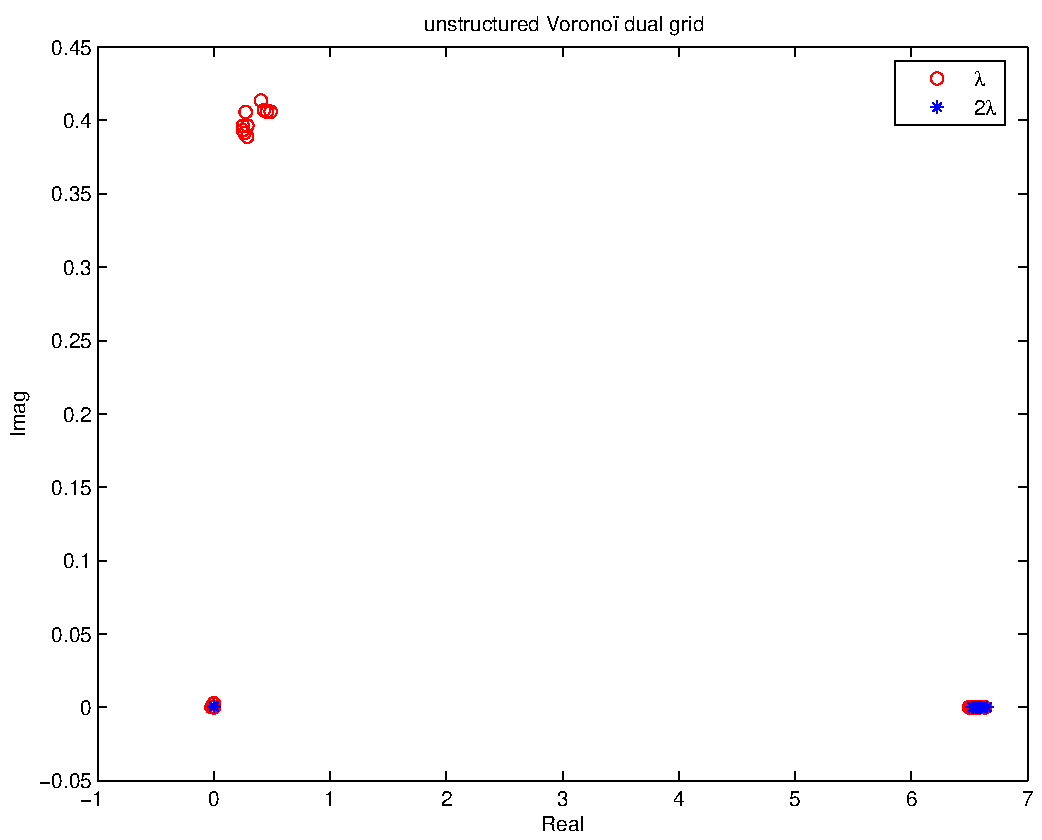
\includegraphics[width=5cm]{pics/eigvals_lambda}}
    \subfigure[Structured and unstructured grids give approximately the
    same eigenvalues, but for unstructured grid they are more
    clustered.]{\label{fig:eigvals:unstructured}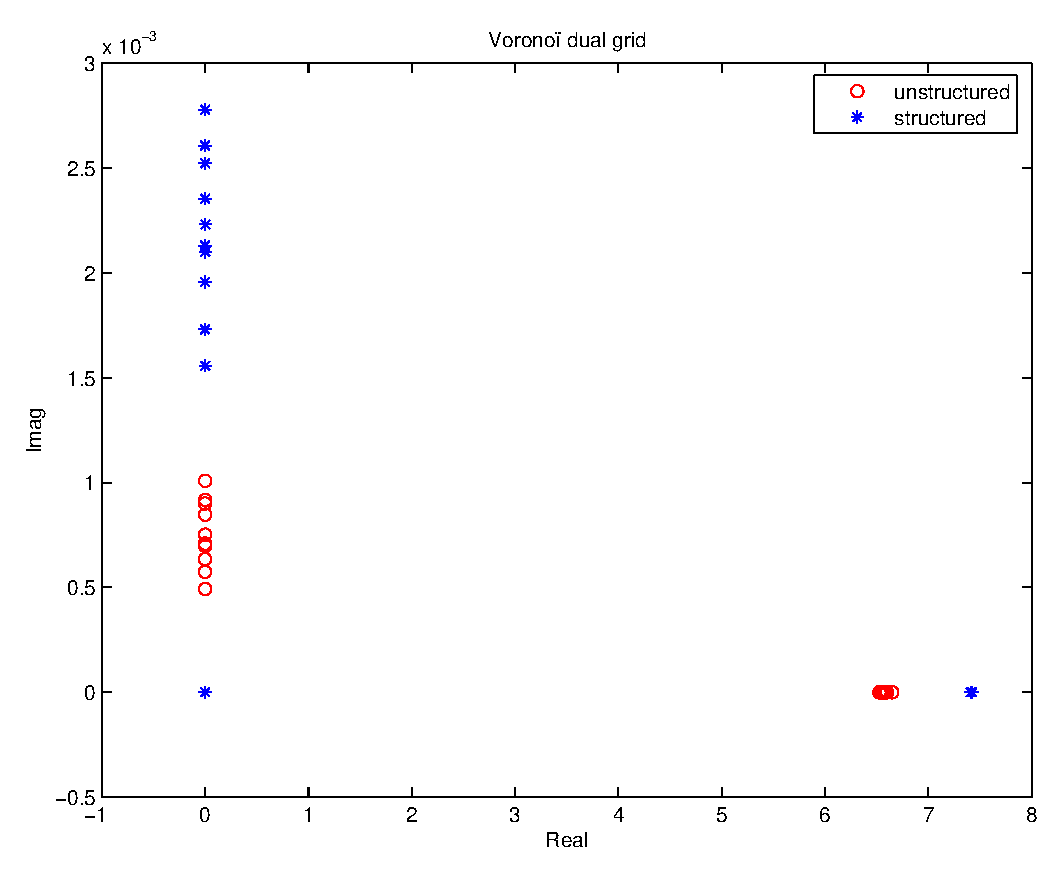
\includegraphics[width=5cm]{pics/eigvals_unstructured}}
    \subfigure[Without PMLs all the eigenvalues are
    real.]{\label{fig:eigvals:pml}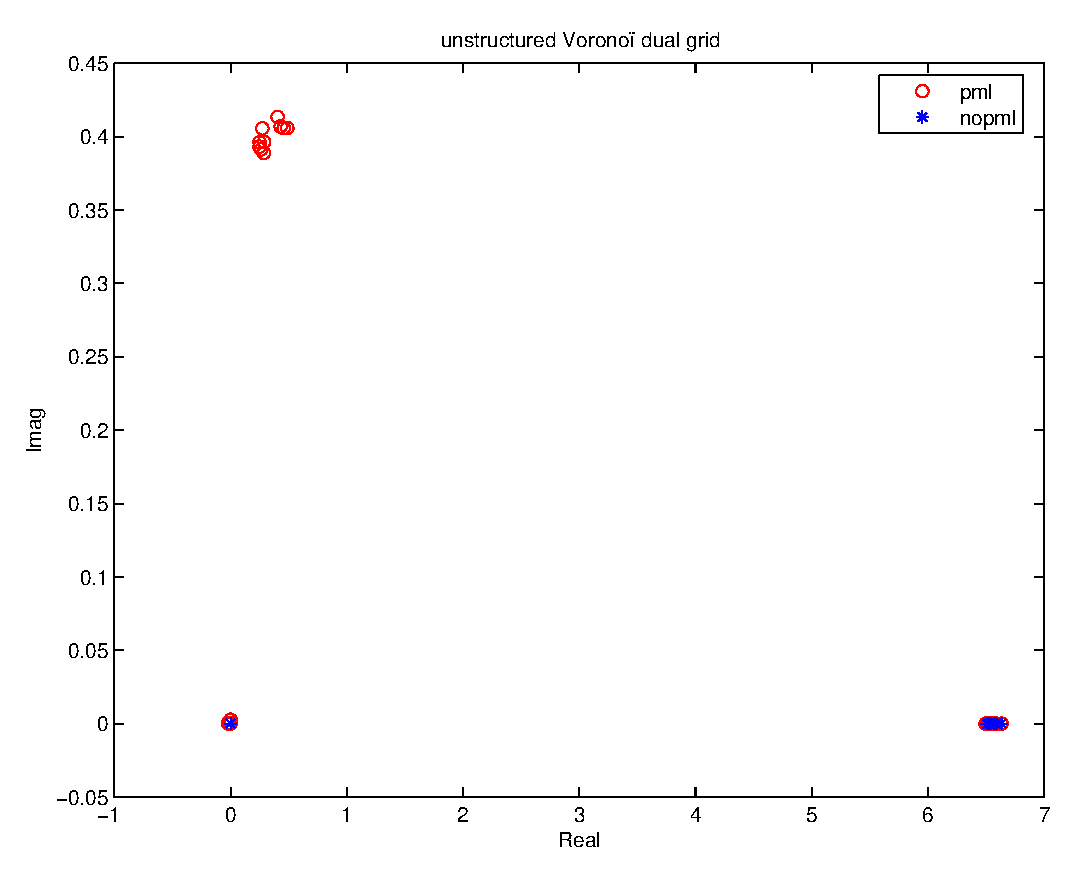
\includegraphics[width=5cm]{pics/eigvals_pml}}
  \end{center}
  \caption{Eigenvalues of the system matrix, for
    different possible parameters, listed in
    \tabref{tab:frequency_parameters}.}
  \label{fig:eigvals}
\end{figure}  

The algorithm has been applied to both two-dimensional and
three-dimensional problems. As said before, most of two-dimensional
problems can be extremely efficiently solved with direct methods. If
iterative methods are applied, most of them tend to give decent
performances (not comparable to direct methods, though): only few do
not converge to the exact result.

For three-dimensional problems, the situation is drastically
different. For the much increased complexity of the problem (more
non-zero elements fraction, bigger matrices, divergenceless property of
the magnetic field not automatically satisfied, more challenging
preconditioners), only very few iterative methods seem to converge. In
particular, many experiments have shown that the most effective
iterative solver is the QMR\index{Methods!iterative!QMR} with Jacobi preconditioning\index{Preconditioning!Jacobi}.

\begin{description}
\item[QMR] is very effective for non-Hermitian sparse linear systems
  \cite{freund_qmr,freund_implementation,freund_iterative,kilmer_qmr},
  so for the kind of problem we face in our formulation;
\item[Jacobi preconditioning]\index{Preconditioning!Jacobi} is effective for strongly diagonal
  matrices because it uses as a preconditioner $\Matrix{P}$ just the
  diagonal of the system matrix.

  It doesn't achieve good convergence speed, but it's definitely
  stable and it is well defined also from strongly indefinite
  matrices, while others preconditioners (like the ILU) are not.
\end{description}

\section{Examples}

\subsection{2-D}

Photonic crystals are a typical example of a two-dimensional problem
in which the present method is particularly effective. The particular
circular shape of the scatterers of the photonic crystal used enhances
the advantage of having an unstructured grid over a structured one
\cite{cangellaris_analysis}.

\figref{fig:2d_channel:mesh} shows the mesh for a two-dimensional photonic crystal
channel. The dielectric scatterers are air holes in a dielectric
substrate (refractive index $n = 3.0$), with lattice period $\Lambda =
0.5 \mu m$ and radius $R = 0.35 \Lambda$. Only the TE polarization is
studied, for which the photonic crystal presents a
bandgap\footnote{The value of the refractive index have no specific
  meaning: it has been chosen so that the photonic crystal has a
  bandgap for the given $\lambda$, $\Lambda$ and $R$. Studying a
  highly resonant frequency -- like one in the bandgap -- is a tougher
  problem than a non-resonant one.}.

\figref{fig:2d_channel:matrix} shows the system matrix obtained for
the frequency domain problem, for a Vorono\"i\index{Vorono\"i} dual grid. We can note
that it is sparse, with a symmetric non-zero pattern and strongly
diagonal. Its dimension is $49795 \times 49795$, with $346532$
non-zero elements: only $0.1398\%$ of the elements are non-zero. Its
sparsity pattern is a direct indication of the node numbering used by
the meshing software used to generate the mesh \cite{triangle}.

\figref{fig:2d_channel:bcgs} and \figref{fig:2d_channel:gmres} show
the convergence of two iterative methods used to solve the problem:
the BiCGStab and the GMRES, as implemented in the PETSc\index{PETSc} library
\cite{petsc}. The stopping criterion is a value of the residual below
$10^{-7}$. We can note that GMRES achieves convergence within $4000$
steps (a number of iterations about $1.15\%$ of the dimension of the
system matrix!) with the Eisenstat \cite{petsc} and the ILU
preconditioning: the convergence is fairly exponential in these
cases. For other preconditioners, the convergence is not so rapid, and
sub-exponential. Without preconditioning the algorithm tends to
stagnate. The BiCGStab, on the other hand, achieves convergence faster
(after about $3000$ steps, with the same preconditioners), but it's
much more irregular.

\begin{figure}[htbp]
  \begin{center}
    \subfigure[Primary mesh. In black are the circular scatterers, in
    blue, on the left, a plane wave source at a fixed $\lambda$ and in
    green, on the right, a sensor to collect the output fields.]{\label{fig:2d_channel:mesh}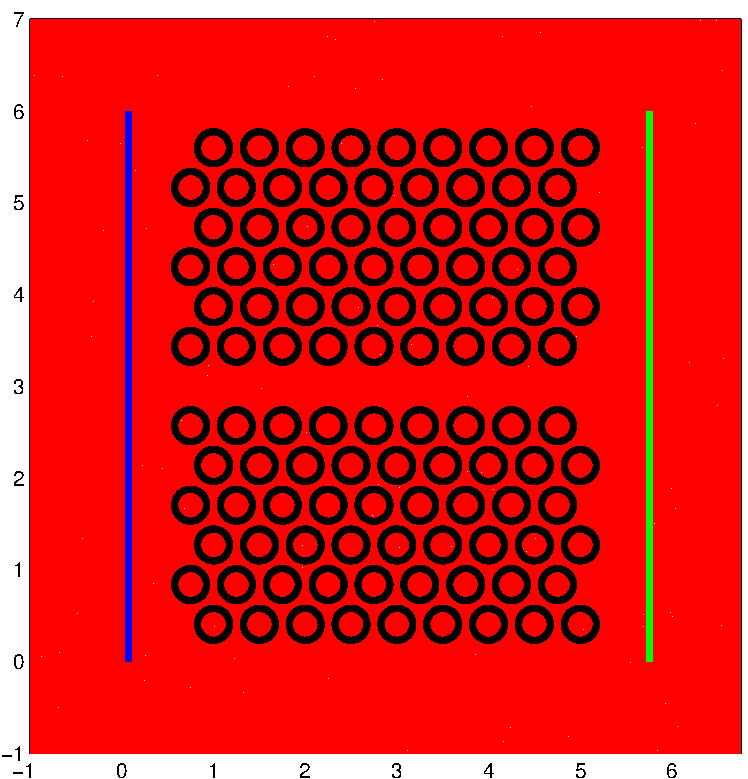
\includegraphics[width=6cm]{pics/channel_mesh}}
    \subfigure[System matrix. Only $0.1398\%$ of the
    elements are non-zero.]{\label{fig:2d_channel:matrix}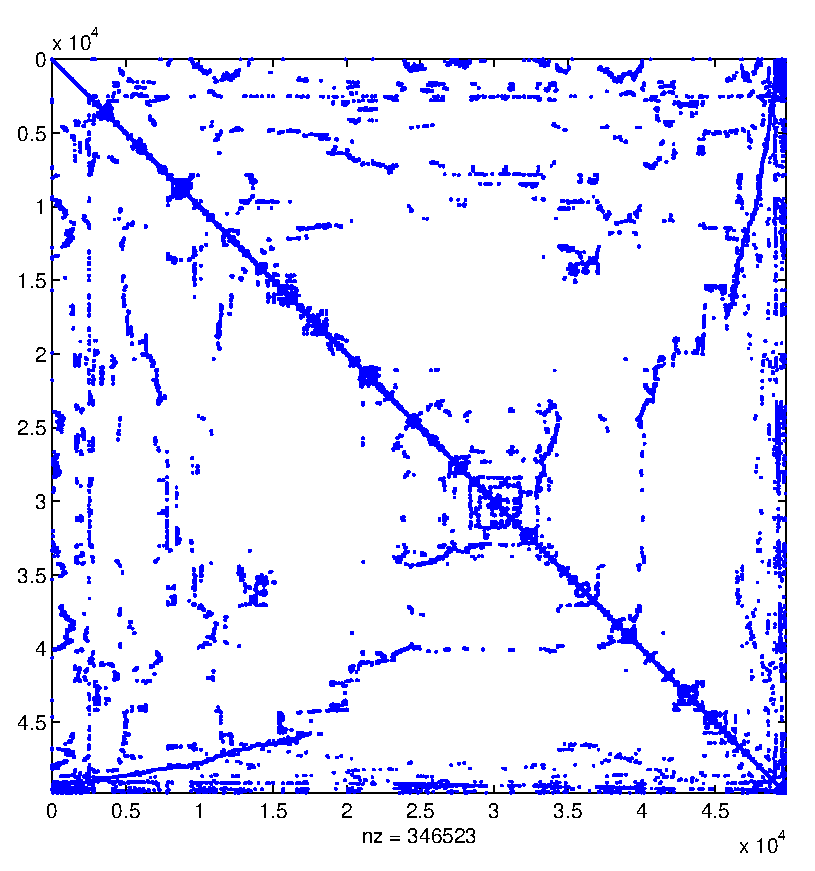
\includegraphics[width=6cm]{pics/channel_M}}
    \subfigure[Convergence of the BiCGStab algorithm to the exact
      solution for different preconditioners. The best result is
    achieved with the Eisenstat preconditioner, a particular type of
    SOR preconditioner \cite{petsc}.]{\label{fig:2d_channel:bcgs}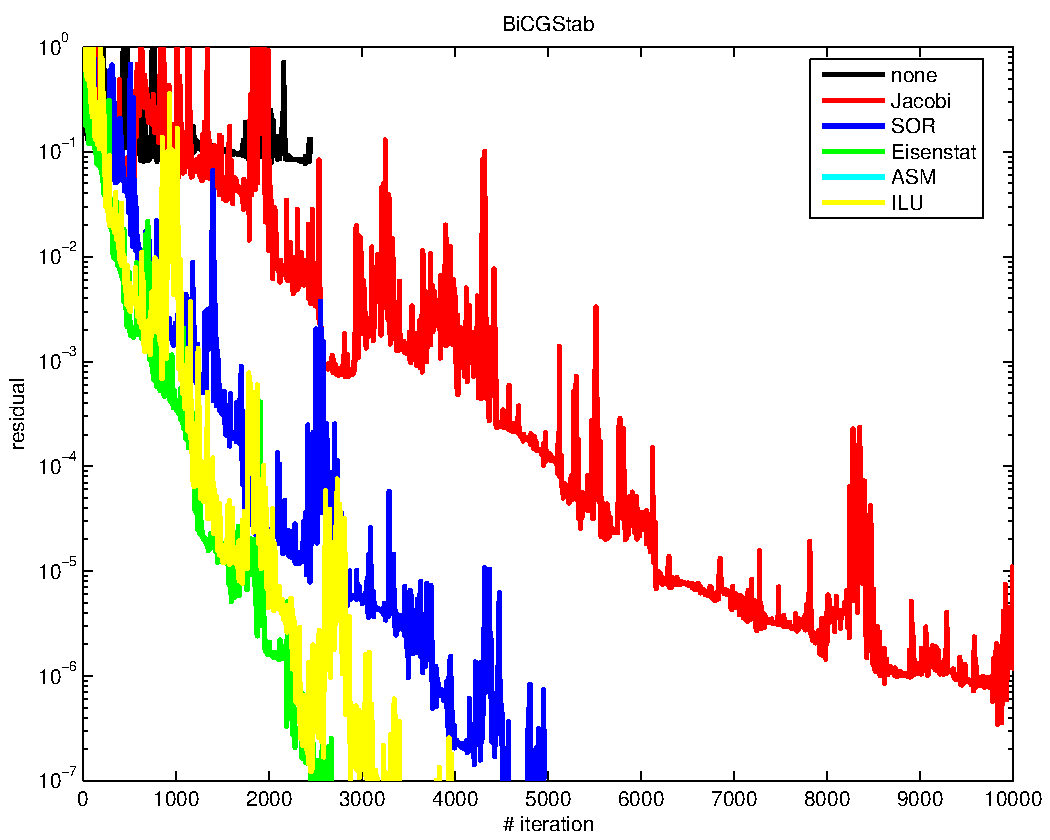
\includegraphics[width=6cm]{pics/channel_convergence_bicgstab}}
    \subfigure[Convergence of the GMRES algorithm to the exact
    solution for different preconditioners. Note that the convergence
    is much smoother than for the BiCGStab.]{\label{fig:2d_channel:gmres}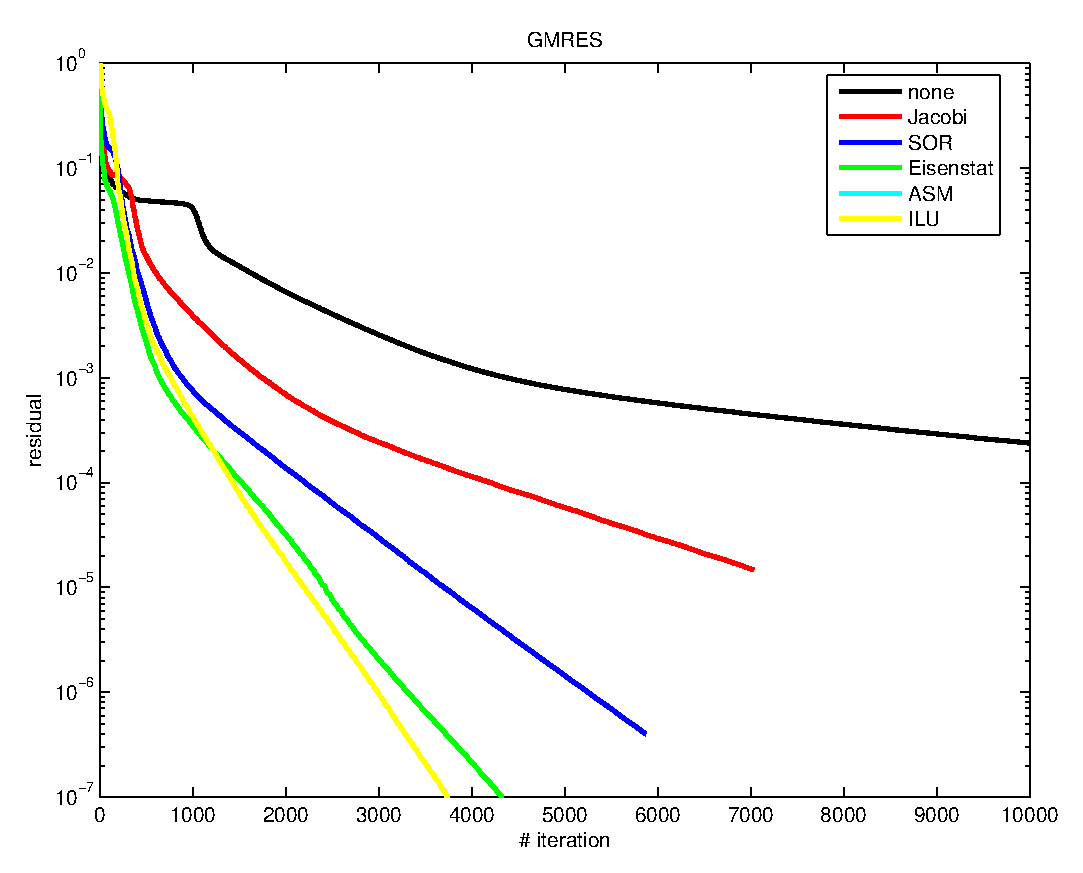
\includegraphics[width=6cm]{pics/channel_convergence_gmres}}
  \end{center}
  \caption{Two-dimensional example: photonic crystal channel.}
  \label{fig:2d_channel}
\end{figure}

Note that the memory requirements for same problem allow to solve it
using direct methods \cite{umfpack}. In this case, the performances of
the algorithm are definitely superior: the direct solver gives an
exact\footnote{Exact, within the numerical precision of the computer used.}
solution in few seconds, compared to few minutes of the iterative
solver.

Another interesting example is the study of a photonic crystal
Y-junct\-ion: see \figref{fig:Yjunct}. The lattice is triangular with a
period $\Lambda = 430 nm$, made of holes of radius $R = 0.30 \Lambda$
in a substrate of GaAs/AlGaAs.  The big problem of these devices is
that for the classical triangular lattice of air holes on a silicon
substrate, bends are usually lossy. Light must then be ``helped'' to
bend by arranging the holes in a proper way. Thank to its high speed
when a direct solver is chosen, the two-dimensional algorithm has
been employed with the help of the commercial optimizer Kallistos
\cite{kallistos}, to verify the best position for the scatterers and
achieve the highest power transmission\footnote{The first optimization
has been carried out with FIMMWAVE \cite{fimmwave} and Kallistos
\cite{kallistos}.}. The simulations, even if two-dimensional, have
been used to model a real three-dimensional structure, using the
\emph{effective index method}\index{Effective!index!method}. The complete three-dimensional
structure has also been built, by the University of St. Andrews, and a
very promising $75\%$ transmission has been measured over $110nm$ at
$\lambda = 1.55 \mu m$ \cite{ayre_experimental}.

\begin{figure}[htbp]
  \begin{center}
    \subfigure[Optimized position of the scatterers. The lattice
    period is $\Lambda = 430 nm$ and the radius of the scatterers is
    $R = 0.30 \Lambda$.]{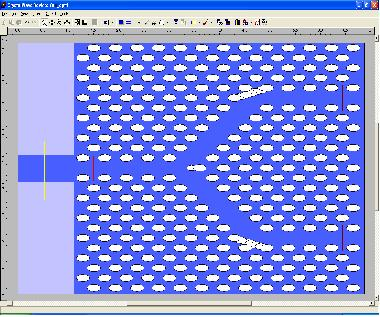
\includegraphics[width=6cm]{pics/Yjunct}}
    \subfigure[Power in the
    device. Note the ``steering'' effect of the holes in the
    Y-junction bends.]{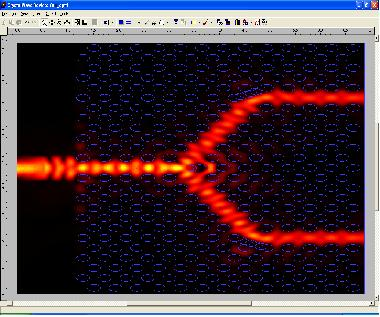
\includegraphics[width=6cm]{pics/Yjunct_field}}
  \end{center}
  \caption{Two-dimensional example: a photonic crystal Y-junction.}
  \label{fig:Yjunct}
\end{figure}

\subsection{3-D} \label{sec:frequency_domain:3D}

Two examples of three-dimensional devices are reported here.

\subsubsection{Metallic Waveguide}

First, the propagation in a metallic waveguide is studied. This
device, extremely simple from a theoretical point of view, permits to
compare the analytical solution with the computed one and have an
exact reference.

The waveguide, shown in \figref{fig:simple_waveguide_geom}, is a
rectangular waveguide, with cross section of $\sqrt{3} \times 1\,\mu
m^2$ and a length of $6\,\mu m$, full of air. The working wavelength
is $\lambda = \sqrt{3}\,\mu m$, for which the waveguide is
monomodal. The metallic walls are perfect and PMLs are present only at
the beginning and at the end, to simulate an infinitely long
waveguide. The computational domain correspond to the waveguide
itself. The fundamental mode $TE_{1,0}$, known from theory, is excited
from one end.

\begin{figure}[htbp]
  \begin{center}
    \resizebox{6cm}{!}{\input{pics/simple_waveguide.pdf_t}}
  \end{center}
  \caption{Three-dimensional example: geometry of a metallic waveguide.}
  \label{fig:simple_waveguide_geom}
\end{figure}

After the discretization of \figref{fig:simple_waveguide_mesh}, the
system matrix dimension is $174839 \times 174839$, with $2005449$
non-zero elements (see \figref{fig:simple_waveguide_M}). The
``block-diagonal'' non-zero pattern is easily explained by the
three-dimensional mesh used and the numeration of nodes chosen: a
two-dimensional extruded mesh, already mentioned in
\secref{sec:mesh:orientation}. The numbering of nodes is fixed by the
meshing software \cite{triangle} in each ``floor'', and this explains
the internal nonzero pattern of each block in the matrix, but it's
ordered between one ``floor'' and the next: this explains the block
diagonal pattern. In a sense, each single layer is a block of the
matrix, plus some entries that are the edges linking the ``floors''
each others.

\begin{figure}[htbp]
  \begin{center}
    \subfigure[Example of a mesh layer in the extruded three-dimensional grid.]{\label{fig:simple_waveguide_mesh}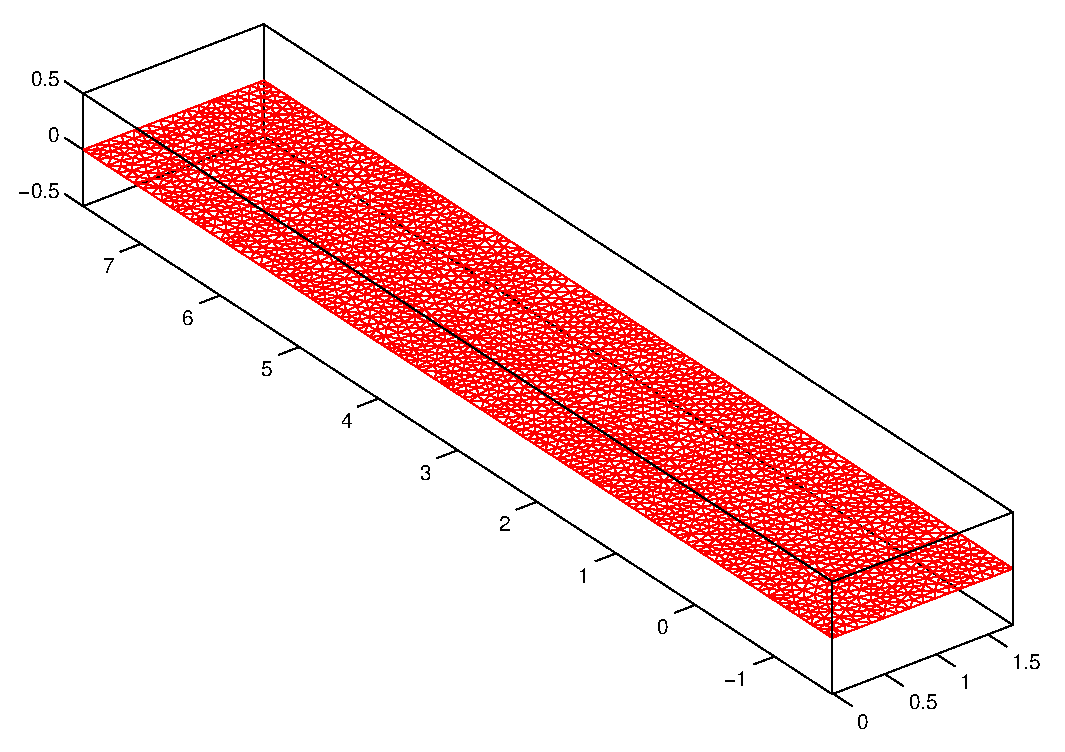
\includegraphics[width=6cm]{pics/simple_waveguide_mesh}}
    \subfigure[System matrix.]{\label{fig:simple_waveguide_M}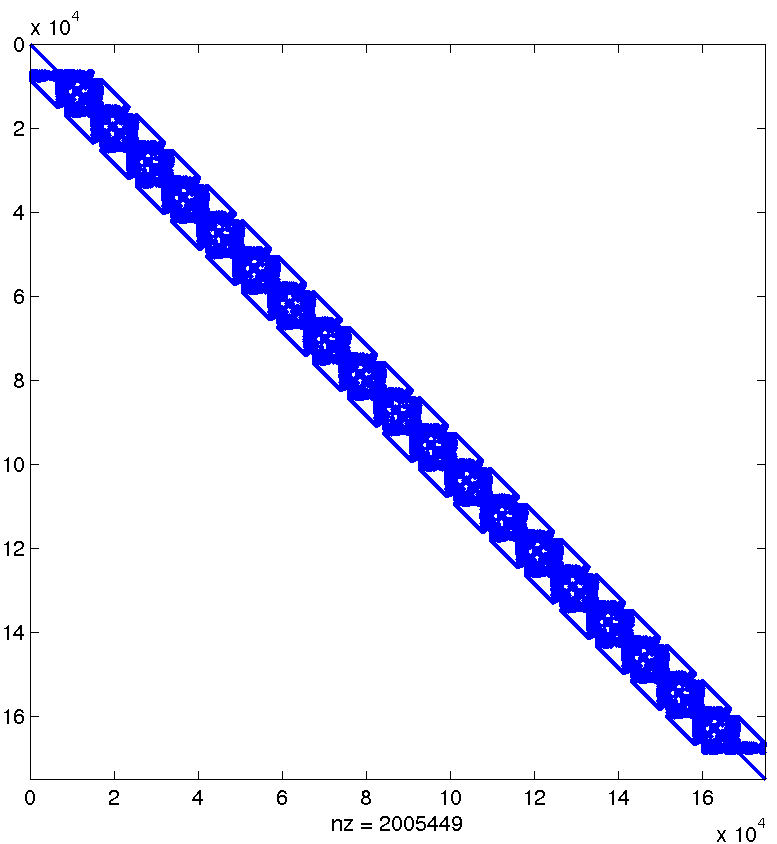
\includegraphics[width=6cm]{pics/simple_waveguide_M}}
    \subfigure[GMRES convergence.]{\label{fig:simple_waveguide_gmres}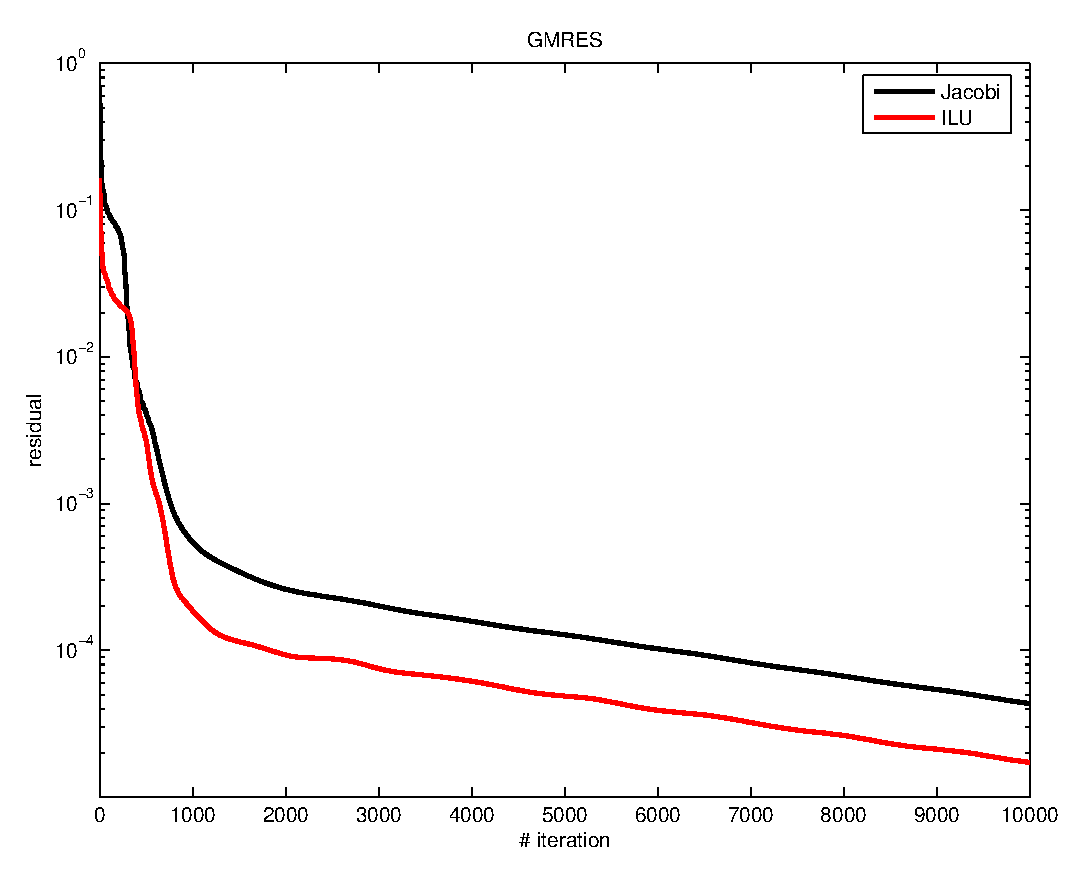
\includegraphics[width=6cm]{pics/simple_waveguide_convergence_gmres}}
    \subfigure[QMR with Jacobi preconditioner convergence.]{\label{fig:simple_waveguide_qmr}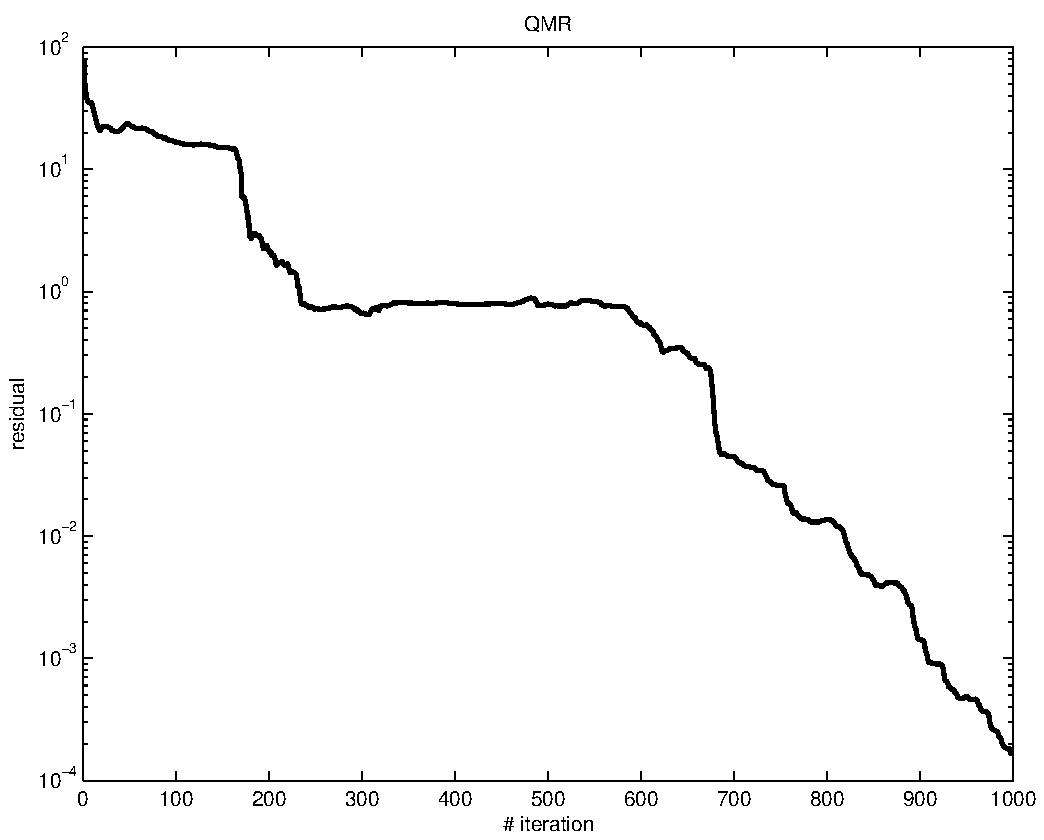
\includegraphics[width=6cm]{pics/simple_waveguide_convergence_qmr}}
  \end{center}
  \caption{Three-dimensional example: the metallic waveguide.}
  \label{fig:simple_waveguide}
\end{figure}

\begin{figure}[htbp]
  \begin{center}
    \subfigure[$\Real{E_z}$ in a $z$-constant section: theoretical and computed.]{\label{fig:simple_waveguide_section_z}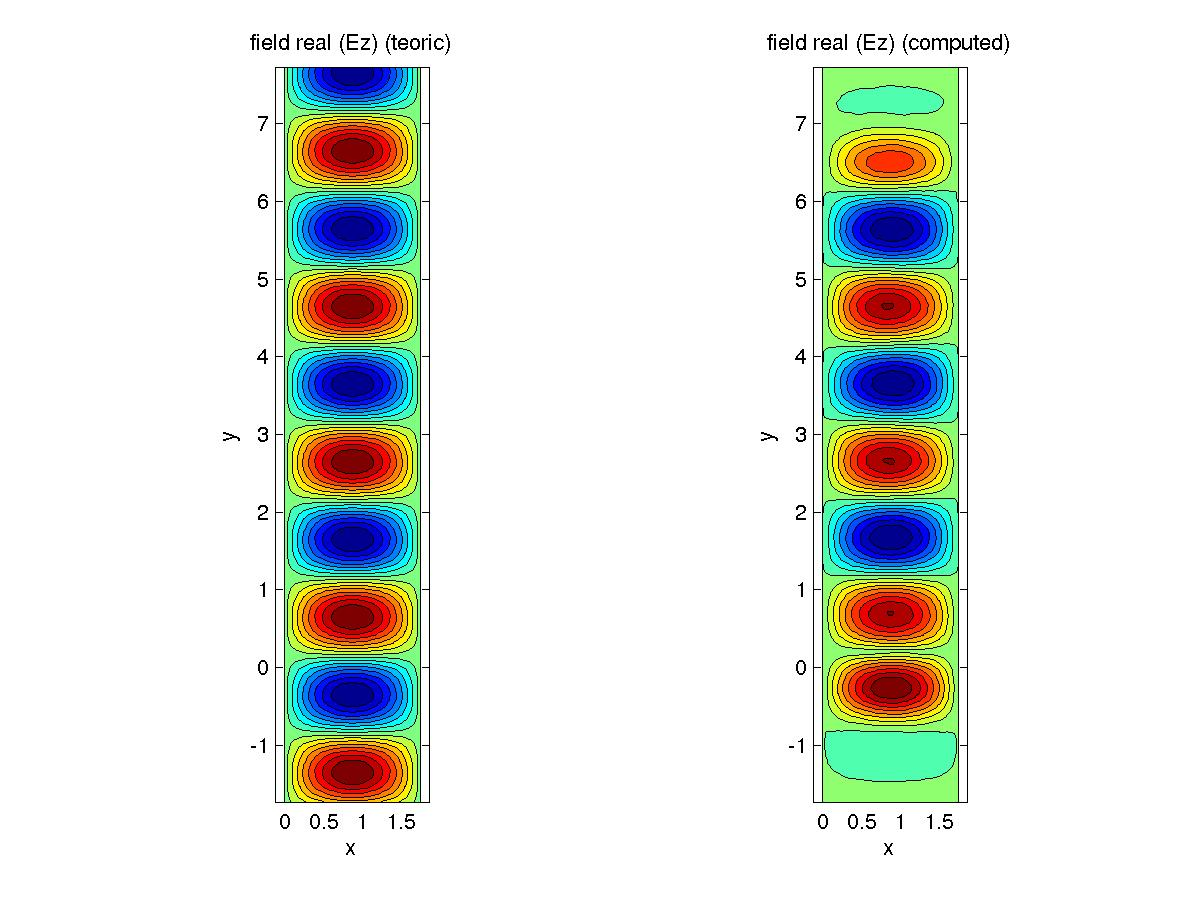
\includegraphics[width=6cm]{pics/simple_waveguide_Ez_real_section_z}}
    \subfigure[$\Real{E_z}$ in a $xz$-constant section: theoretical and
    computed. Black lines shows the PMLs; the red line, the $TE_{1,0}$
    mode source. Comparison is meaninful only outside the PMLs.]{\label{fig:simple_waveguide_section_xz}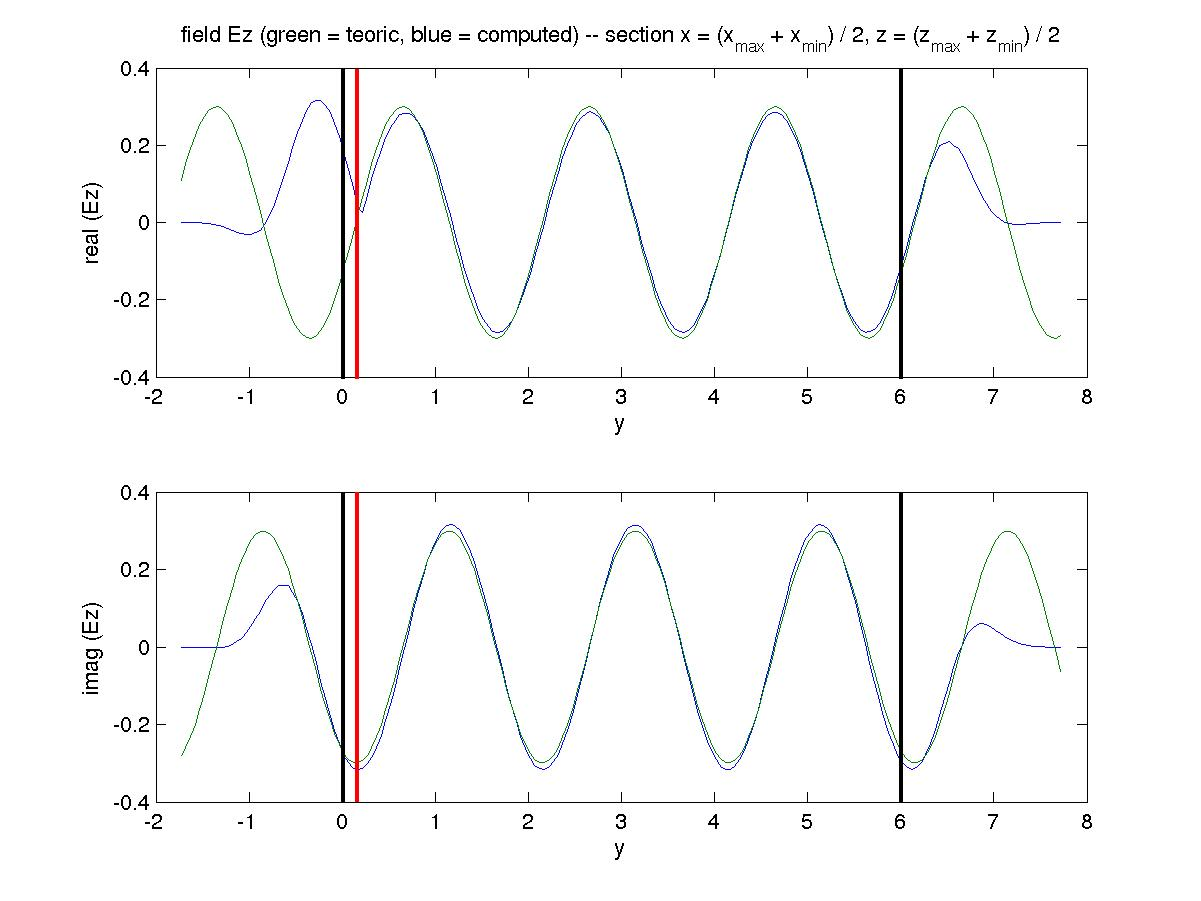
\includegraphics[width=6cm]{pics/simple_waveguide_Ez_section_xz}}
  \end{center}
  \caption{Three-dimensional example: resulting fields for the metallic waveguide.}
  \label{fig:simple_waveguide_section}
\end{figure}

\figref{fig:simple_waveguide_gmres} shows the convergence of the GMRES
algorithm with two possible preconditioners: Jacobi and ILU. Neither
of them give good results: after ten thousand steps, the residual is
still above $10^{-5}$. A better convergence, even if more irregular,
is given by the QMR algorithm with Jacobi preconditioner, shown in
\figref{fig:simple_waveguide_qmr}. It achieves the same residual of
the GMRES, but in one tenth of the steps.

The solution obtained is shown and compared to the theoretical one in
\figref{fig:simple_waveguide_section_z} and
\figref{fig:simple_waveguide_section_xz}. The standard deviation $\sigma$,
defined as the square root of the mean value of the squared distance
between theoretical and computed values, sampled in $N$ points, is
never above $1\%$. In formulas:
\begin{equation} \label{eqn:standard_deviation}
  \sigma = \sqrt{\frac{1}{N} \sum_N\left(\Abs{E_z^{\text{computed}}} -
  \Abs{E_z^{\text{theoretical}}}\right)^2} \leq 1\%
\end{equation}

\subsubsection{Planar Photonic Crystal Channel}

A more challenging example is shown in
\figref{fig:uniud_phc_coarse}. It is the simulation of a Gaussian
pulse propagating inside a three-dimensional photonic crystal channel.

The photonic crystal is made of a $1\,\mu m$ thick dielectric slab ($n
= 3.0$) with $1\,\mu m$ deep air holes. A line defect uses the bandgap
of the structure to guide the light through the device.

The absolute value of the $z$-component of electric field computed is
shown in \figref{fig:uniud_phc_coarse_field}.

\figref{fig:uniud_phc_coarse_M} shows the system matrix: again, the
numbering of each layer is visible. Note that the non-zero elements
are $8$ millions: this is a device by far bigger than any commercial
software is able to simulate. Thanks to the present formulation, the
unstructured grid and an efficient iterative method, the solution is
found after $5000$ steps, with a precision below $10^{-6}$. The whole
simulation took few hours over a Pentium III computer.

\begin{figure}[htbp]
  \begin{center}
    \subfigure[System matrix: it presents more than $8$ million non-zeros.]{\label{fig:uniud_phc_coarse_M}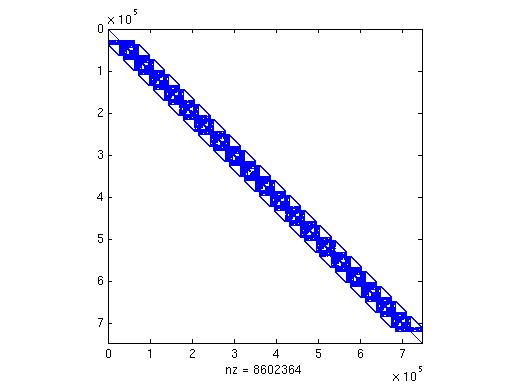
\includegraphics[width=6cm]{pics/uniud_phc_coarse_M}}
    \subfigure[QMR with Jacobi convergence.]{\label{fig:uniud_phc_coarse_residual}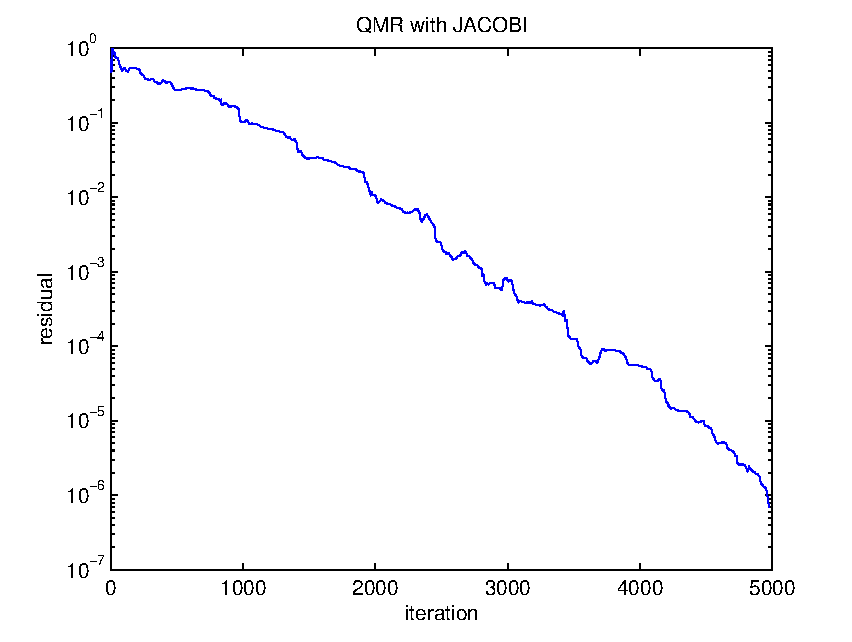
\includegraphics[width=6cm]{pics/uniud_phc_coarse_RESVEC}} \\
    \subfigure[$\Abs{E_z}$ on a $z$-constant section.]{\label{fig:uniud_phc_coarse_field}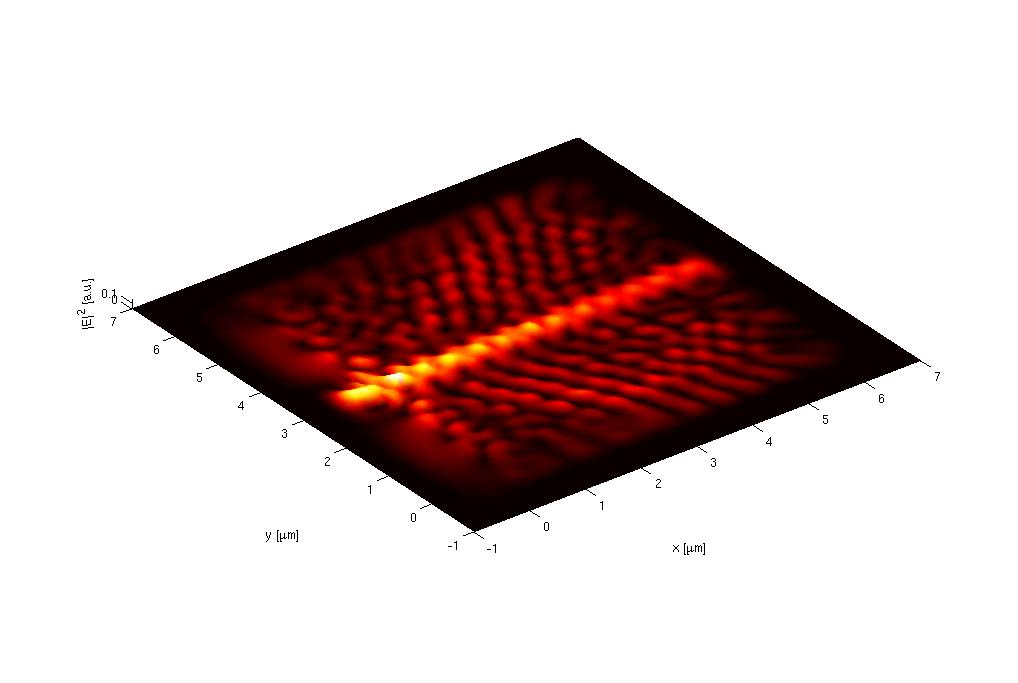
\includegraphics[width=12cm]{pics/uniud_phc_coarse}}
  \end{center}
  \caption{Three-dimensional example: planar photonic crystal channel.}
  \label{fig:uniud_phc_coarse}
\end{figure}  

\section{Validation of the method}

Validation of the method has been worked out by comparison with the
commercial software FIMMPROP \cite{fimmprop} by Photon
Design\index{Photon Design} \cite{photond}: the analysis is particular
useful because FIMMPROP uses a completely different algorithm, based
on the Eigenmode Expansion technique\index{Eigenmode Expansion}.

The choice of the problems for the validation has been guided by the
will to test situations where our algorithm has advantages over the
Eigenmode Expansion technique. For this reason, photonic crystals have
been chosen.

The validation is done by the study of three problems:
\begin{description}
\item[free-space propagation]: this problem has been used as a
  ``calibration'' test, to have a feel of convergence and accuracy as
  well as of the normalization constants between the two algorithms;
\item[single scatterer]: this problem has been used to highlight
  possible advantages of the present method in case of circular
  scatterers, where staircase approximation (done by the Eigenmode
  Expansion technique) can lead to bad performances;
\item[photonic crystal channel]: this is a complete test, for which
  the Eigenmode Expansion technique is not the best solution.
\end{description}

\figref{fig:validation_01}, \figref{fig:validation_02} and
\figref{fig:validation_03} show the domain of the three validation
tests. The yellow line on the left-hand side is always the input,
which is a Gaussian pulse. The red lines are \emph{output sensors}, in
which fields are collected and compared.

Comparison is done by the calculation of the standard deviation,
defined in \eqref{eqn:standard_deviation}.

\subsection{Free-space propagation} \label{sec:validation_01}

The first validation test is studied mainly to calibrate the two
algorithms, i.e. to find possible numerical constants implicitly
included in the computed fields, ``tune'' the PMLs and test the
results on a very simple problem. \figref{fig:validation_01_domain}
shows the computational domain: a $6 \times 1.5\,\mu m^2$ empty
rectangle. The source is a Gaussian beam, $w = 1\,\mu m$ width, at
$\lambda = 1.55\,\mu m$: with this choice of $\lambda$ and $w$,
diffraction is clearly visible. Fields are collected on the red lines,
with the most left-hand sided used as a reference for the other one.

\figref{fig:validation_01_convergence} shows the quadratic error
between FIMMPROP and our algorithm, as a function of the grid
density. The different curves on the graph refer to different PMLs
parameters in FIMMPROP.

We can note that the results tend to converge to the same value,
within $0.2\%$ of tolerance for a $30$ points-per-wavelength mesh
density. For a mesh $15$ points-per-wavelength density, the standard
deviation is already below $1\%$: the algorithm tends to converge very
rapidly to a good solution and then any refinement is very slow. The
reason can also be a non-perfect convergence of FIMMPROP's result,
which showed difficulties with PMLs.

The field collected at the output sensor is shown in
\figref{fig:validation_01_field}: we can note its Gaussian shape,
larger than at the input for the effect of diffraction. The little
wobbling at the boundaries of the domain confirms the non-perfect
tuning of the PMLs.

\begin{figure}[htbp]
  \begin{center}
    \subfigure[Computational domain.]{\label{fig:validation_01_domain}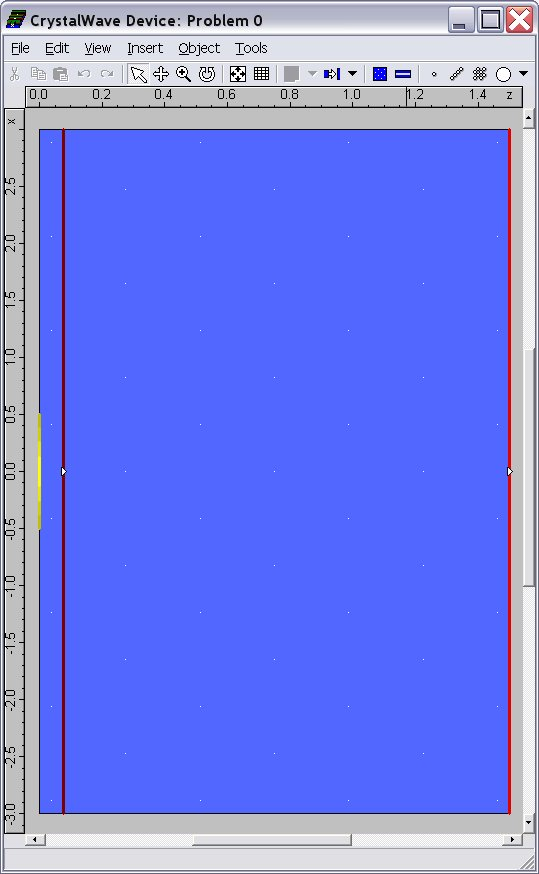
\includegraphics[height=6cm]{pics/validation_01}}
    \subfigure[Convergence to the reference solution.]{\label{fig:validation_01_convergence}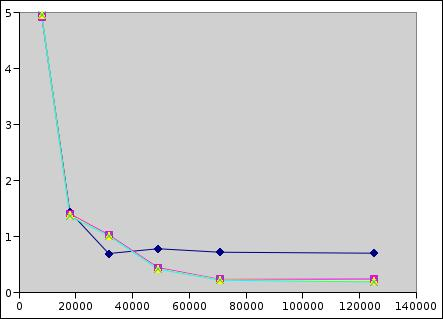
\includegraphics[height=6cm,width=6cm]{pics/validation_01_convergence}}
    \subfigure[Absolute value of the magnetic field on the most
    right-hand sided output sensor, for different mesh grids.]{\label{fig:validation_01_field}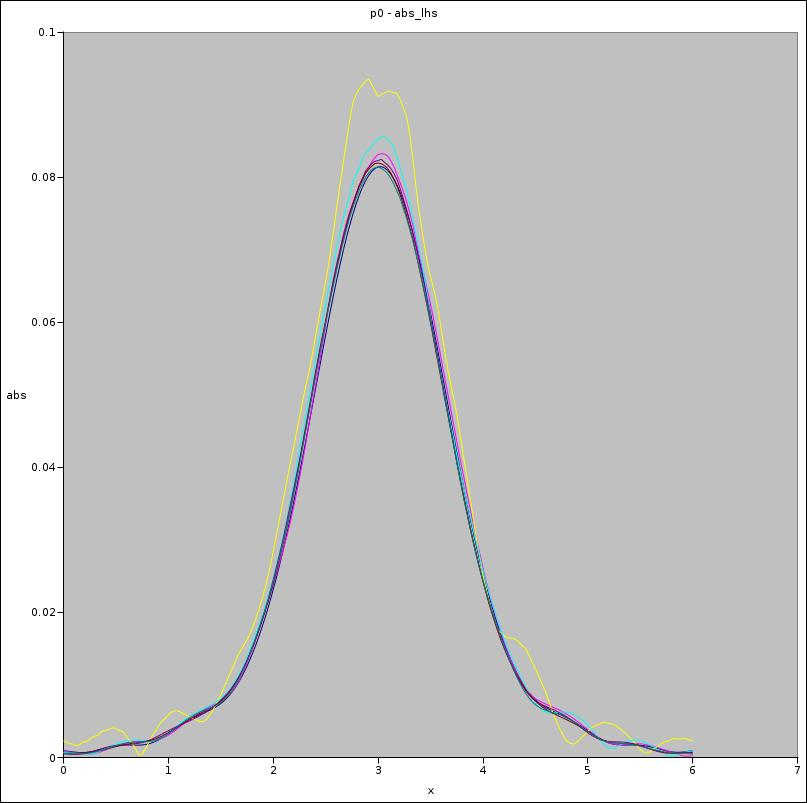
\includegraphics[height=6cm,width=6cm]{pics/validation_01_field}}
  \end{center}
  \caption{Free-space propagation.}
  \label{fig:validation_01}
\end{figure}  

\subsection{Single scatterer} \label{sec:validation_02}

The second validation test, whose computational domain is shown in
\figref{fig:validation_02}, is the diffraction of a Gaussian pulse by
a dielectric scatterer. The domain's geometry is the same as in
\ref{sec:validation_01}. The dielectric scatterer is a circle filled
with air, in a dielectric domain with refractive index $n = 3.0$.

This time, a preliminary PMLs optimization in FIMMPROP has been done,
and the results are shown in
\figref{fig:validation_02_fimmwave}. Different lines refer to
different PML thicknesses\footnote{It is not always true that the
  thicker the PML, the best the result: in algorithms based on modal
  expansion, the exponentially increasing modes inside the PMLs can
  lead to numerical instabilities. The tradeoff is, of course, between
the numerical instability of a too thick PML layer and the poor
absorption of a too thin one.}.

\figref{fig:validation_02_convergence} and
\figref{fig:validation_02_field} show the convergence to the reference
solution as a function of the mesh density and the output
field. Again, the result converge quickly within $1\%$ and then any
mesh refinement brings little improvement. Note the shadow in the
output field, due to the presence of the dielectric scatterer.

\begin{figure}[htbp]
  \begin{center}
    \subfigure[Computational domain.]{\label{fig:validation_02_domain}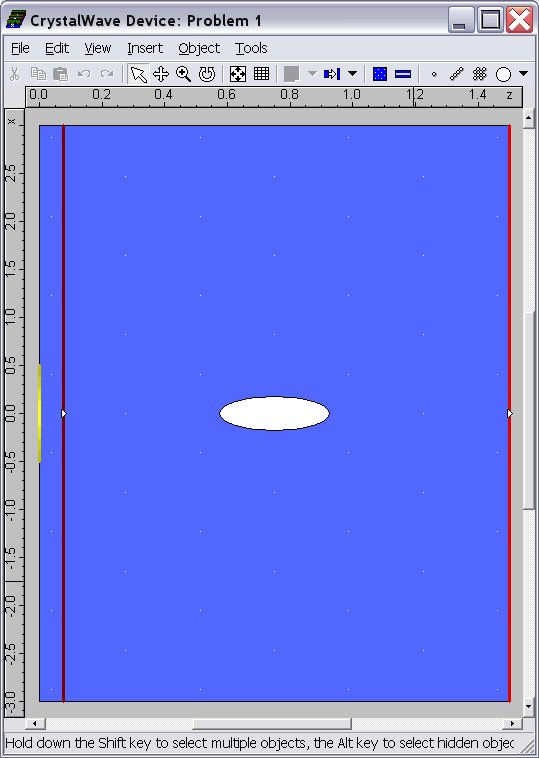
\includegraphics[height=6cm]{pics/validation_02}}
    \subfigure[FIMMPROP PMLs tuning.]{\label{fig:validation_02_fimmwave}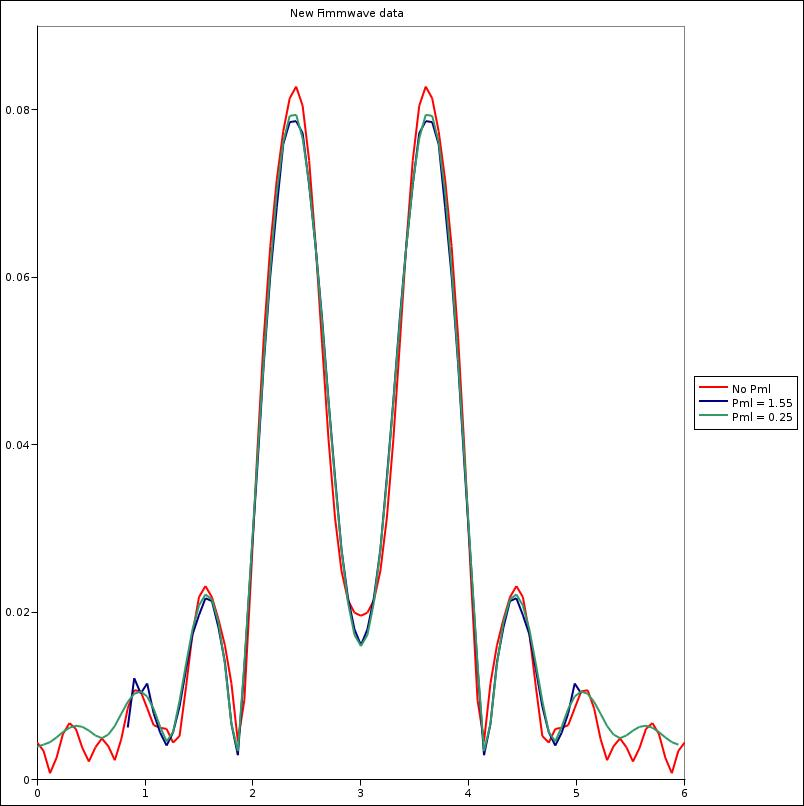
\includegraphics[height=6cm,width=6cm]{pics/validation_02_fimmwave}}
    \subfigure[Convergence to the reference solution.]{\label{fig:validation_02_convergence}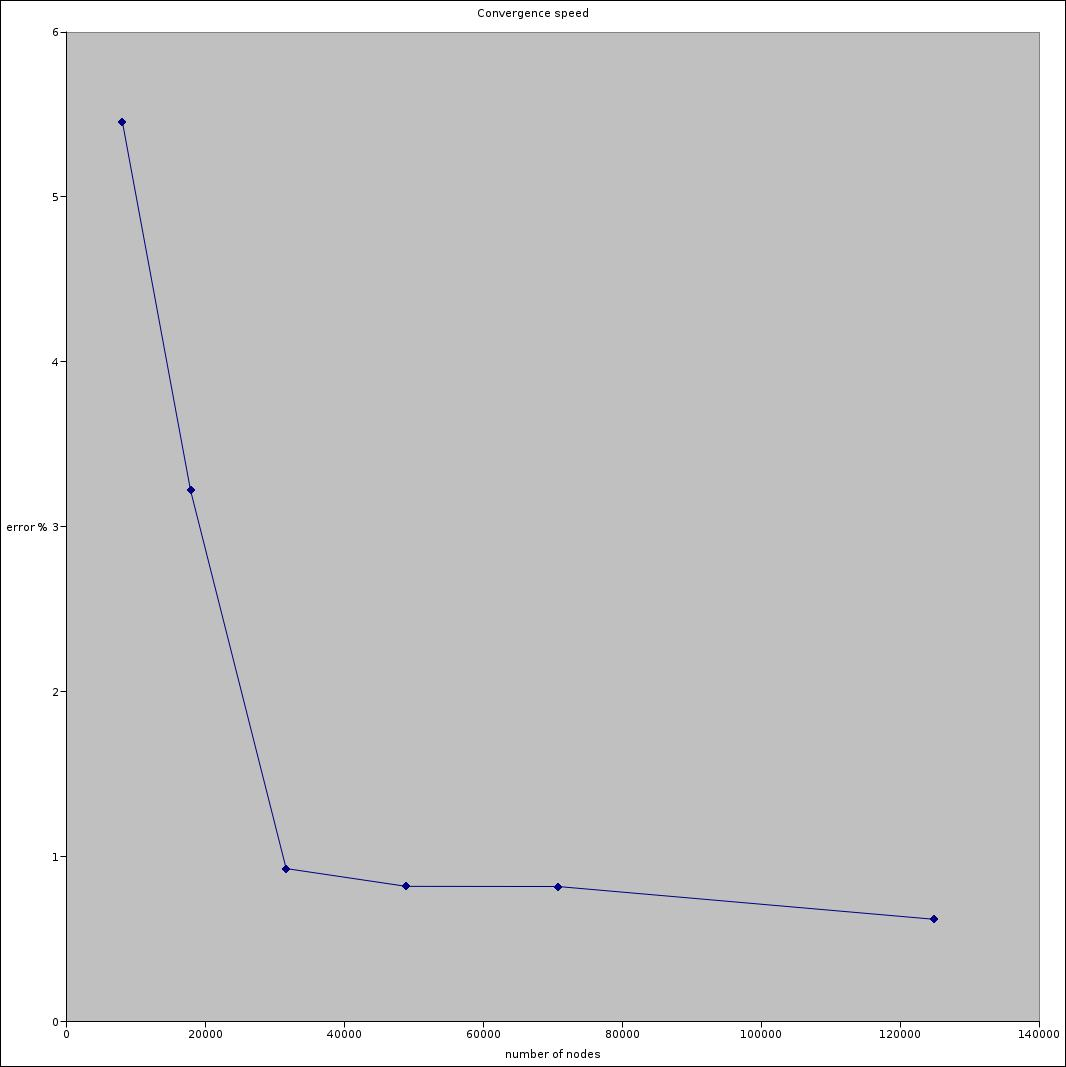
\includegraphics[height=6cm,width=6cm]{pics/validation_02_convergence}}
    \subfigure[Absolute value of the magnetic field on the most
    right-hand sided output sensor, for different mesh grids.]{\label{fig:validation_02_field}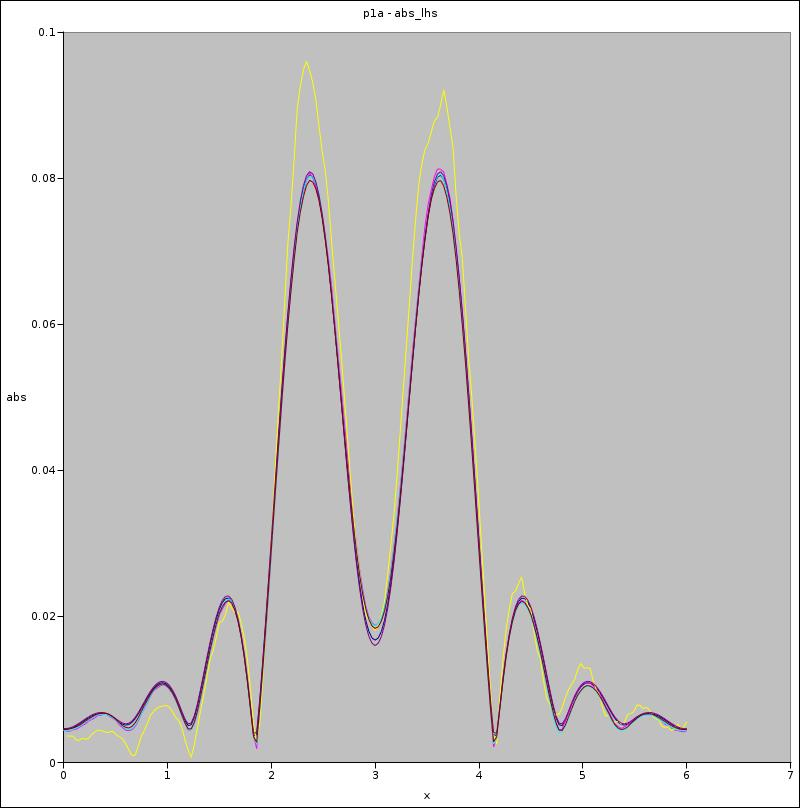
\includegraphics[height=6cm,width=6cm]{pics/validation_02_field}}
  \end{center}
  \caption{Single scatterer.}
  \label{fig:validation_02}
\end{figure}  

\subsection{Photonic Crystal Channel} \label{sec:validation_03}

Finally, \figref{fig:validation_03} shows a complete photonic crystal
channel. The domain is $6 \times 5.75 \mu m^2$, filled with $108$
scatterers as the one studied in \ref{sec:validation_02}, arranged in
a triangular lattice of periodicity $\Lambda = 0.5 \mu m$. A line
defect is left in the lattice to guide the light through the device.

\begin{figure}[htbp]
  \begin{center}
    \subfigure[Computational domain.]{\label{fig:validation_03_domain}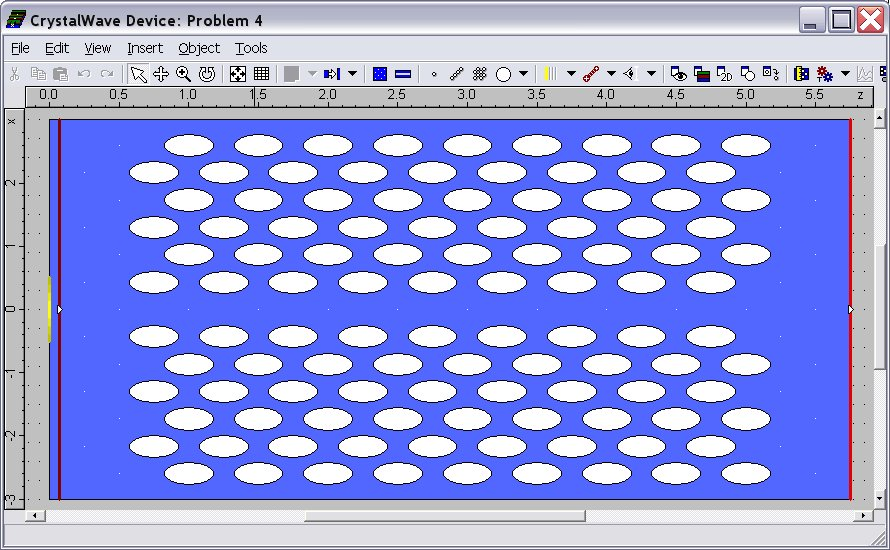
\includegraphics[height=6cm]{pics/validation_03}}
    \subfigure[Absolute value of the magnetic field at the output sensor.]{\label{fig:validation_03_field}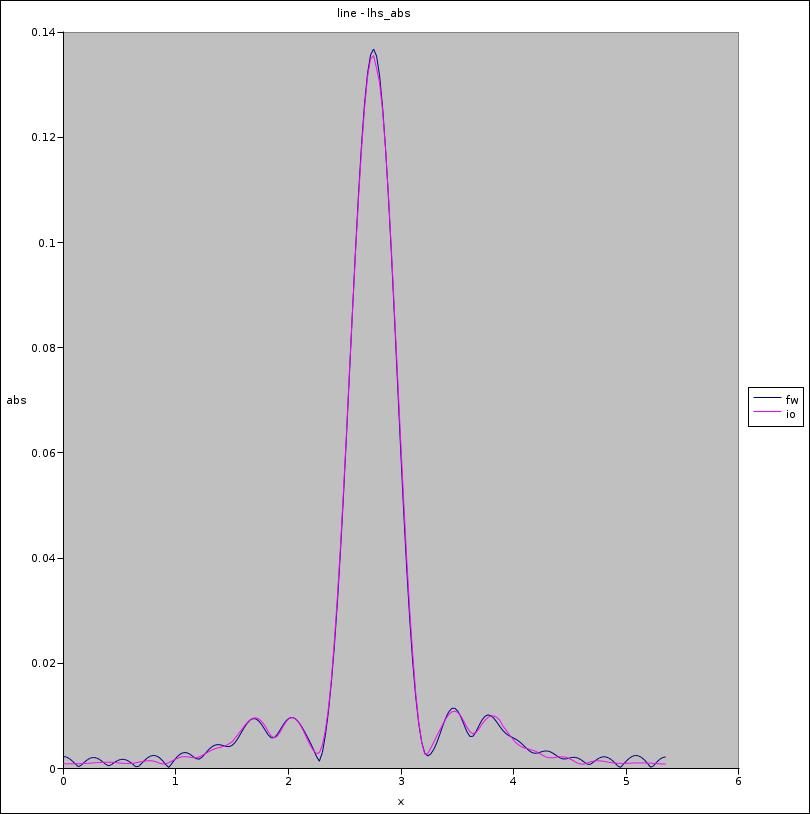
\includegraphics[height=6cm,width=6cm]{pics/validation_03_field}}
    \subfigure[Phase of the magnetic field at the output sensor.]{\label{fig:validation_03_phase}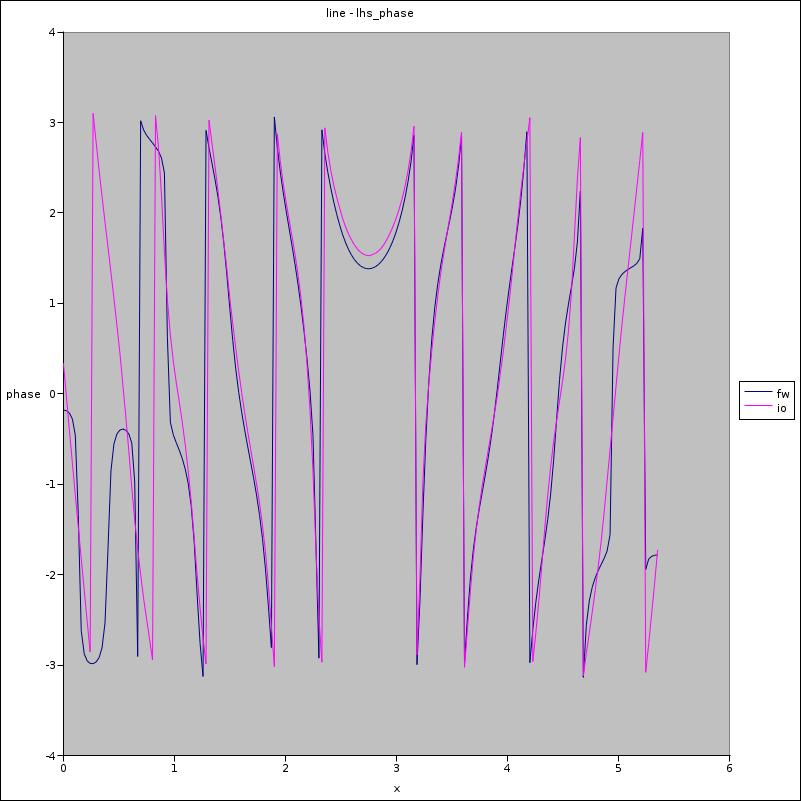
\includegraphics[height=6cm,width=6cm]{pics/validation_03_phase}}
  \end{center}
  \caption{Photonic crystal channel.}
  \label{fig:validation_03}
\end{figure}  

\figref{fig:validation_03_field} and \figref{fig:validation_03_phase}
show the absolute value of the $z$-component of the magnetic field and
its phase at the output sensor. Comparison with FIMMPROP is very good,
except near the boundaries where, to increase the speed and the
accuracy of FIMMPROP, PMLs have been removed. Therefore, comparison makes sense
only away from the boundaries, where the results of the two
algorithms are in good agreement.









%% \OKKIO{mostrare dove il
%%   residuo e' massimo: PML... e' li' che gli autovalori fanno fatica a
%%   ``convergere''...}

%% \section{FDFD}
%% blah

%% \subsection{Setting Up the Sources}
%% Equivalence Theorem

%% \section{FEFD}
%% discretizzazione/riduzione vs riduzione/discretizzazione

%% \subsection{PML}
%% stima empirica dei parametri ottimali

%% \subsection{Setting Up the Sources}
%% Equivalence Theorem

%% \subsection{Matrix Properties}
%% \begin{itemize}
%% \item
%%   indefiniteness.pdf
%% \item
%%   symmetry.pdf
%% \item
%%   eigvals.pdf
%% \end{itemize}

%% \OKKIO{It can be shown that the eigenvalues of $\Matrix{D}$ lie on a
%%   circumference of unitary radius: as $\deltat \rightarrow 0$, the
%%   circumference becomes smaller and smaller and the eigenvalues fall
%%   into the unitary circle.}

